
\subsection{Nguồn 1: Spotify Top 50 Playlist Songs }

\begin{itemize}
    \item     \textbf{Link dataset: }https://www.kaggle.com/datasets/anxods/spotify-top-50-playlist-songs-anxods
    \item     \textbf{Link github: }https://github.com/minhnhut273/spotify-data-project
\end{itemize}

\subsubsection{Giới thiệu dữ liệu}
  \textbf{Tổng quan} 


    - Bộ dữ liệu cung cấp thông tin bài hát nằm trong bảng xếp hạng Top 50 của Spotify của một số quốc gia gồm 9 nước (United States, Spain, United Kingdom, Italy, France, Mexico, Argentina, Japan, South Korea) và 1 bảng xếp hạng chung top 50 trên thế giới.

  
    - Phạm vi dữ liệu ngoài vị trí địa lý còn về mặt thời gian bộ dataset cung cấp nằm trong khoảng 05/2023 đến 11/2024.

   \textbf{Một số đặc trựng ban đầu:}

\begin{itemize}
    \item \textbf{date}: Ngày thu thập dữ liệu hoặc ngày xếp hạng. 


    \item \textbf{position}: Vị trí của bài hát trong bảng xếp hạng Top 50. 


    \item \textbf{song}: Tên bài hát. 


    \item \textbf{artist}: Tên nghệ sĩ hoặc nhóm nghệ sĩ chính. 


    \item \textbf{popularity}: Chỉ số phổ biến (Spotify popularity score, 0–100). 


    \item \textbf{duration\_ms}: Độ dài bài hát tính bằng mili-giây. 


    \item \textbf{album\_type}: Loại album chứa track này (ví dụ: album, single, compilation). 


    \item \textbf{total\_tracks}: Tổng số track trong album chứa bài hát đó. 


    \item \textbf{release\_date}: Ngày phát hành album (chứa bài hát này).

    \item \textbf{is\_explicit}: Cho biết bài hát có nội dung 18+ hay không. 
   

    \item \textbf{album\_cover\_url}: Link ảnh bìa album.
\end{itemize}

\begin{figure}[h] % môi trường figure để quản lý hình
    \centering % căn giữa
    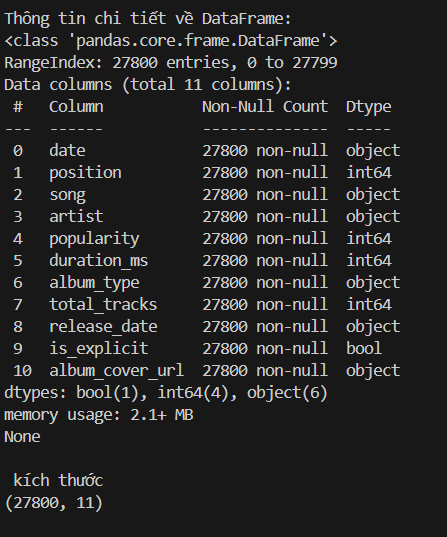
\includegraphics[width=0.5\textwidth]{../graphics/data_top50/raw.png} % tên file hình
    \caption{Đặc điểm chung của các dataset} % chú thích
    \label{fig:example} % nhãn để tham chiếu
\end{figure}
\textbf{=> Kết quả có được 10 file spotify-streaming-top-50-{region}.csv có đặc điểm như hình trên}

 \subsubsection{Bổ sung dữ liệu:}

 \textbf{- Dùng Spotify API để hoàn thiện metadata}
 \\ 
 \begin{itemize}
     \item \textbf{Giới thiệu API:} Spotify Web API là dịch vụ do Spotify cung cấp. Cho phép lập trình viên truy cập dữ liệu nhạc số trên Spotify, hoạt động qua HTTP request (RESTful API). 
     \item \textbf{Mục đích:} Do nhóm nhận thấy các trường dữ liệu của dataset gốc chưa cung cấp đầy đủ, chi tiết về metadata của dữ liệu nên nhóm quyết định sử dụng API này để hoàn thiện nó.
     \item \textbf{Các trường có thể thêm gồm:}
    \begin{itemize}
        \item \textbf{track\_id}: ID duy nhất của bài hát trên Spotify.
        \item \textbf{album\_id}: ID duy nhất của album chứa bài hát.
        \item \textbf{uri}: Định danh Spotify URI (dùng để mở trực tiếp trong Spotify).
        \item \textbf{href}: Link API đến resource (track/album) trong Spotify Web API.
        \item \textbf{external\_url}: Link mở trên Spotify (dành cho người dùng).
        \item \textbf{external\_ids}: Thông tin định danh khác (ví dụ ISRC – mã nhận dạng bản ghi).
        \item \textbf{disc\_number}: Số đĩa (trong trường hợp album nhiều đĩa).
        \item \textbf{track\_number}: Vị trí bài hát trong album/đĩa.
        \item \textbf{release\_date\_precision}: Độ chính xác của ngày phát hành (có thể là year, month, hoặc day).
        \item \textbf{is\_playable}: Cho biết bài hát có thể phát được không (True/False).
        \item \textbf{linked\_from}: Nếu bài hát được liên kết từ một track khác (ví dụ bản sao trong album khác).
        \item \textbf{preview\_url}: Link nghe thử 30 giây bài hát.
        \item \textbf{restrictions}: Các giới hạn (ví dụ chỉ phát được ở một số quốc gia).
        \item \textbf{available\_markets}: Danh sách quốc gia mà track này có sẵn.
        \item \textbf{genres}: Thể loại âm nhạc nghệ sĩ theo đuổi.
    \end{itemize}
 \end{itemize}
 
\begin{figure}[h] % môi trường figure để quản lý hình
    \centering % căn giữa
    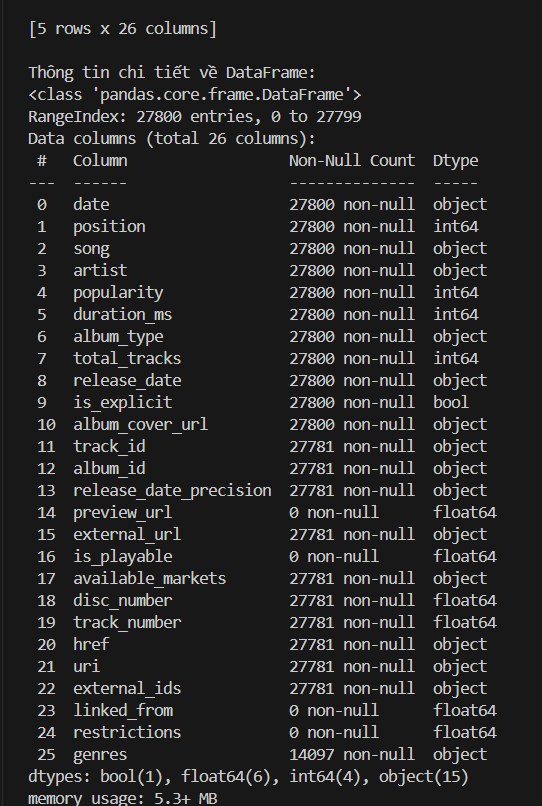
\includegraphics[width=0.5\textwidth]{../graphics/data_top50/figure/script/raw_meta/Screenshot 2025-09-30 225603.png} % tên file hình
    \caption{Các trường sau khi thêm} % chú thích
    \label{fig:example} % nhãn để tham chiếu
\end{figure}

\textbf{=> Kết quả có được các file ..with-meta.csv có đặc điểm như hình trên}

\begin{itemize}
    \item \textbf{Hạn chế:} Tuy nhiên, do một số chính sách mới ra cuối năm 2024 của Spotify dẫn đến các nhóm người không thể truy cập được một số nội dung ( chart, lyric,...) trong đó có audio feature - nguồn dữ liệu mà nhóm quan tâm.
\end{itemize}
\textbf{- Dùng ReccoBeats để bổ sung audio feature: }
\begin{itemize}
    \item \textbf{Giới thiệu API:}Recobeats API là một dịch vụ bên thứ ba giúp lấy dữ liệu nhạc từ Spotify (playlist, audio features, metadata) và dùng cho phân tích hoặc gợi ý nhạc. Tuy nhiên nó không phải API chính thức.
    
    % , nên có thể bị giới hạn hoặc phụ thuộc vào quyền truy cập Spotify. 
    \item \textbf{Các trường có thể thêm: }
    \begin{itemize}
    \item \textbf{href}: Link Spotify đến bài hát (https://open.spotify.com/track/<track\_id>). Dùng để mở hoặc kiểm tra thủ công.
    \item \textbf{acousticness}: Mức độ “mộc” (0.0–1.0). Cao => nhạc acoustic, ít electronic.
    \item \textbf{danceability}: Độ dễ nhảy (0.0–1.0). Cao => dễ nhảy, dựa trên nhịp, groove, tempo.
    \item \textbf{energy}: Cường độ/độ bốc (0.0–1.0). Liên quan tới tempo, loudness, mật độ âm thanh.
    \item \textbf{instrumentalness}: Khả năng không lời (0.0–1.0). >0.5 thường là nhạc cụ/không lời.
    \item \textbf{key}: Tông nhạc (0–11, -1 nếu không phát hiện). Ví dụ: 0=C, 1=C\#/Db, … 11=B. 
    \item \textbf{liveness}: Dấu hiệu biểu diễn live (0.0–1.0). >0.8 thường là bản live.
    \item \textbf{loudness}: Độ ồn trung bình (dB, -60 => 0). Giá trị càng gần 0 càng to. 
    \item \textbf{mode}: Điệu thức: 1 = Major (tươi sáng), 0 = Minor (trầm buồn). 
    \item \textbf{speechiness}: Tỷ lệ lời nói (0.0–1.0). >0.66: chủ yếu là nói; 0.33–0.66: rap/spoken; <0.33: chủ yếu là nhạc.
    \item \textbf{tempo}: Nhịp độ (BPM, 0–250). Nhạc phổ biến: 60–200 BPM.
    \item \textbf{valence}: Độ “tươi vui”/tích cực (0.0–1.0). 0.0 = buồn/tối, 1.0 = vui/sáng.
    \end{itemize}

\end{itemize}

\begin{figure}[h] % môi trường figure để quản lý hình
    \centering % căn giữa
    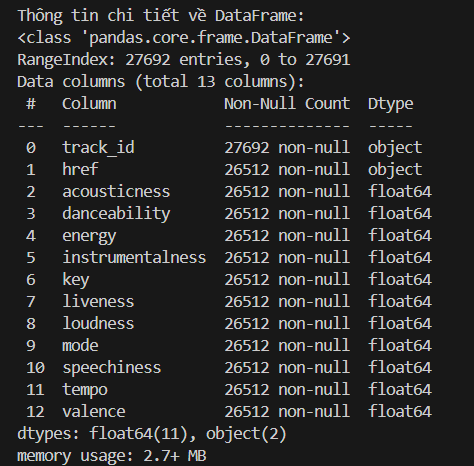
\includegraphics[width=0.5\textwidth]{../graphics/data_top50/figure/script/raw_audio/Screenshot 2025-09-30 230213.png} % tên file hình
    \caption{Bảng đặc trưng} % chú thích
    \label{fig:example} % nhãn để tham chiếu
\end{figure}

    \textbf{=> Kết quả có các file ..with-audio.csv có đặc điểm như hình trên}








% \subsubsection{Tiền xử lý }

% \textbf{- Xử lí Metadata: }

% \begin{itemize}
%     \item \textbf{Giữ lại một số trường  cần thiết:}
      
% \begin{itemize}

%     % Giữ lại một số trường cần thiết:
%     \begin{itemize}
%         \item \textbf{date}  phân tích theo thời gian.
%         \item \textbf{position} => vị trí xếp hạng trong Top 50.
%         \item \textbf{song} => tên bài hát.
%         \item \textbf{artist} => tên nghệ sĩ.
%         \item \textbf{track\_id} => khóa chính để join với with-audio.
%         \item \textbf{popularity} => đo mức độ phổ biến.
%         \item \textbf{duration\_ms} => độ dài bài hát (có thể phân tích thêm).
%         \item \textbf{is\_explicit} => xem tỷ lệ nhạc explicit.
%         \item \textbf{album\_id} => phân tích theo album (nếu cần).
%         \item \textbf{release\_date} => phân tích mới/cũ.
%         \item \textbf{genres} => phân tích xu hướng thể loại.
%     \end{itemize}

%     % Bỏ các trường không cần thiết:
%     \item \textbf{Bỏ:}
%     \begin{itemize}
%         \item \textbf{album\_type}, \textbf{total\_tracks} => chỉ mô tả album.
%         \item \textbf{release\_date\_precision} => nếu không phân tích độ chính xác ngày phát hành.
%         \item \textbf{album\_cover\_url}, \textbf{preview\_url}, \textbf{external\_url}, \textbf{uri}, \textbf{href}, \textbf{external\_ids} => chỉ để hiển thị/mở nhạc.
%         \item \textbf{is\_playable}, \textbf{available\_markets}, \textbf{disc\_number}, \textbf{track\_number}, \textbf{linked\_from}, \textbf{restrictions}  không cần cho phân tích.
%     \end{itemize}

% \end{itemize}
% \end{itemize}
% \begin{itemize}
%     \item  \textbf{Xử lý Missing Values (Data Cleaning)}
%     \begin{itemize}
%         \item \textbf{Mục tiêu:} đảm bảo dữ liệu không còn NaN ở các cột quan trọng.
%         \item \texttt{track\_id:} nếu thiếu => điền \texttt{"unknown\_track"} (không xóa để giữ dữ liệu phân tích).
%         \item \texttt{album\_id:} nếu thiếu => \texttt{"unknown\_album"}.
%         \item \texttt{release\_date:}
%         \begin{itemize}
%             \item Nếu chỉ có năm => ghép \texttt{"YYYY-01-01"}.
%             \item Nếu NaN => cũng dùng \texttt{"YYYY-01-01"} dựa trên năm nhỏ nhất trong cột \texttt{date}.
%         \end{itemize}
%         \item \texttt{genres:} nếu NaN => \texttt{"unknown"}.
%         \item \textbf{ Kết quả:} file mới không còn dòng NaN cho \texttt{track\_id}, \texttt{album\_id}, \texttt{release\_date}, \texttt{genres}.
%     \end{itemize}

%     \item  \textbf{Chuẩn hóa dữ liệu (Standardization)}
%     \begin{itemize}
%         \item \textbf{Mục tiêu:} đưa dữ liệu về format thống nhất để dễ phân tích.
%         \item \texttt{date \& release\_date:}
%         \begin{itemize}
%             \item Convert toàn bộ sang \texttt{datetime} (YYYY-MM-DD).
%         \end{itemize}
%         \item \texttt{genres:}
%         \begin{itemize}
%             \item Nếu nhiều genre => lấy genre đầu tiên làm \texttt{main\_genre}.
%         \end{itemize}
%         \item \texttt{is\_explicit:} Convert về 0/1 (boolean => int).
%         \item \texttt{duration\_ms:} giữ nguyên, chưa cần chia phút/giây.
%         \item \texttt{song, artist:} giữ nguyên, chưa chuẩn hóa.
%         \item \textbf{ Kết quả:} file chuẩn hóa có \texttt{date}, \texttt{release\_date} đúng kiểu ngày, 
%         \texttt{is\_explicit} đồng nhất 0/1, \texttt{main\_genre} rõ ràng cho phân tích.
%     \end{itemize}
% \end{itemize}
%      \textbf{=> Kết quả có được file ..with-meta-clean.csv ở các floder}
    

% \begin{figure}[h] % môi trường figure để quản lý hình
%     \centering % căn giữa
%     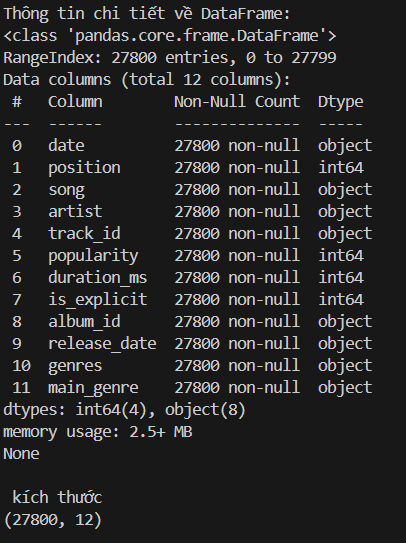
\includegraphics[width=0.5\textwidth]{../graphics/data_top50/figure/script/meta_clean_1/Screenshot 2025-10-02 191458.png} % tên file hình
%     \caption{File meta-clean} % chú thích
%     \label{File meta-clean} % nhãn để tham chiếu
% \end{figure}
% \clearpage


% \textbf{-Xử lí file audio}
% \begin{itemize}
%     \item  \textbf{Bước 1. Kiểm tra \& xử lý Missing Values}
%     \begin{itemize}
%         \item \texttt{track\_id, href:} giữ nguyên (định danh và link).
%         \item \textbf{Các đặc trưng [0–1]} (\texttt{danceability, energy, valence, acousticness, instrumentalness, liveness, speechiness}):
%         \begin{itemize}
%             \item Nếu NaN => thay bằng \textit{median} (hoặc giá trị phổ biến nhất).
%             \item Sau đó clip về \([0,1]\).
%         \end{itemize}
%         \item \texttt{tempo:} 
%         \begin{itemize}
%             \item Nếu NaN hoặc bất thường (\(<30\) hoặc \(>250\)) => thay bằng median.
%         \end{itemize}
%         \item \texttt{loudness:}
%         \begin{itemize}
%             \item Nếu NaN hoặc bất thường (\(<-60\) hoặc \(>0\)) => thay bằng median.
%         \end{itemize}
%         \item \texttt{mode (0/1):} nếu NaN => điền bằng giá trị chiếm đa số trong cột.
%         \item \texttt{key:} 
%         \begin{itemize}
%             \item Nếu \(-1\) hoặc NaN => thay bằng giá trị gần nhất (forward/backward fill hoặc mode).
%             \item Sau đó map sang tên nốt nhạc.
%         \end{itemize}
%     \end{itemize}

%     \item  \textbf{Bước 2. Chuẩn hóa dữ liệu (Standardization)}
%     \begin{itemize}
%         \item \textbf{Các đặc trưng [0–1]} (\texttt{danceability, energy, valence, acousticness, instrumentalness, liveness, speechiness}):
%         \begin{itemize}
%             \item Clip về \([0,1]\), giữ nguyên cột gốc (không thêm).
%         \end{itemize}
%         \item \texttt{tempo:}
%         \begin{itemize}
%             \item Giữ nguyên cột gốc.
%             \item Thêm \texttt{tempo\_norm = (tempo - 30)/(250-30)}.
%         \end{itemize}
%         \item \texttt{loudness:}
%         \begin{itemize}
%             \item Giữ nguyên cột gốc.
%             \item Thêm \texttt{loudness\_norm = (loudness + 60)/60}.
%         \end{itemize}
%         \item \texttt{mode:} giữ nguyên 0/1 (NaN đã được thay).
%         \item \texttt{key:}
%         \begin{itemize}
%             \item Giữ nguyên cột \texttt{key}.
%             \item Thêm cột mới \texttt{key\_name} (C, C\#, D, …, B).
%             \item Đảm bảo không còn \texttt{"unknown"} (đã thay bằng giá trị hợp lệ).
%         \end{itemize}
%     \end{itemize}

%     \item  \textbf{Cột mới sau xử lý:}
%     \begin{itemize}
%         \item \texttt{tempo\_norm} => tempo chuẩn hóa [0,1].
%         \item \texttt{loudness\_norm} => loudness chuẩn hóa [0,1].
%         \item \texttt{key\_name} => tên nốt nhạc thay vì số.
%     \end{itemize}
% \end{itemize}
% \textbf{=> Kết quả ghi đè vào các file ..with-audio.csv}
% \\
%  \begin{figure}[h] % môi trường figure để quản lý hình
%     \centering % căn giữa
%     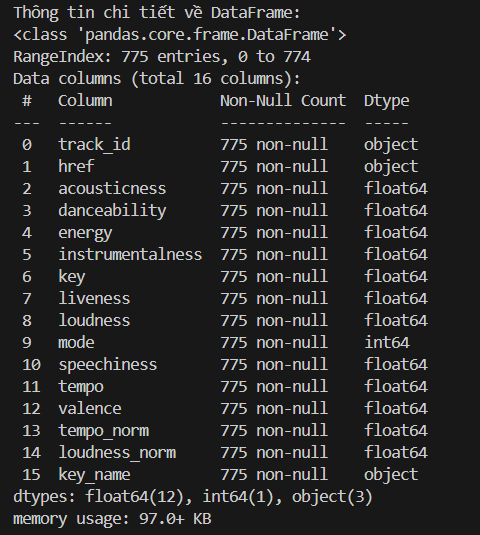
\includegraphics[width=0.75\textwidth]{../graphics/data_top50/figure/script/Screenshot 2025-10-02 192420.png} % tên file hình
%     \caption{File meta-clean} % chú thích
%     \label{File meta-clean} % nhãn để tham chiếu
% \end{figure}
% \clearpage


\subsubsection{Tiền xử lý}

\textbf{- Xử lý Metadata:}

\begin{itemize}
    \item \textbf{Giữ lại một số trường cần thiết:}
    \begin{itemize}
        \item \textbf{date} — phân tích theo thời gian.
        \item \textbf{position} — vị trí xếp hạng trong Top 50.
        \item \textbf{song} — tên bài hát.
        \item \textbf{artist} — tên nghệ sĩ.
        \item \textbf{track\_id} — khóa chính để join với with-audio.
        \item \textbf{popularity} — đo mức độ phổ biến.
        \item \textbf{duration\_ms} — độ dài bài hát (có thể phân tích thêm).
        \item \textbf{is\_explicit} — xem tỷ lệ nhạc explicit.
        \item \textbf{album\_id} — phân tích theo album (nếu cần).
        \item \textbf{release\_date} — phân tích bài mới/cũ.
        \item \textbf{genres} — phân tích xu hướng thể loại.
        \item \textbf{Bỏ các trường không cần thiết còn lại}
    \end{itemize}

    
    % \begin{itemize}
    %     \item \textbf{album\_type}, \textbf{total\_tracks} 
    %     \item \textbf{release\_date\_precision} — nếu không cần độ chính xác ngày phát hành.
    %     \item \textbf{album\_cover\_url}, \textbf{preview\_url}, \textbf{external\_url}, \textbf{uri}, \textbf{href}, \textbf{external\_ids} — chỉ để hiển thị/mở nhạc.
    %     \item \textbf{is\_playable}, \textbf{available\_markets}, \textbf{disc\_number}, \textbf{track\_number}, \textbf{linked\_from}, \textbf{restrictions} — không cần cho phân tích.
    % \end{itemize}
\end{itemize}

\begin{itemize}
    \item \textbf{Xử lý Missing Values (Data Cleaning):}
    \begin{itemize}
        \item \textbf{Mục tiêu:} đảm bảo dữ liệu không còn NaN ở các cột quan trọng.
        \item \texttt{track\_id}, exttt{album\_id} và \texttt{genres} : nếu thiếu $\rightarrow$ điền \texttt{"unknown\_track"}, \texttt{"unknown\_album"} và \texttt{"unknown"}.
        \item \texttt{release\_date:}
        \begin{itemize}
            \item Nếu chỉ có năm $\rightarrow$ ghép \texttt{"YYYY-01-01"}.
            \item Nếu NaN $\rightarrow$ dùng \texttt{"YYYY-01-01"} dựa trên năm nhỏ nhất trong cột \texttt{date}.
        \end{itemize}

    \end{itemize}

    \item \textbf{Chuẩn hóa dữ liệu (Standardization):}
    

    

    \begin{itemize}
        \item \textbf{Mục tiêu:} đưa dữ liệu về format thống nhất để dễ phân tích.
        \item \texttt{date} \& \texttt{release\_date:}
        \begin{itemize}
            \item Convert toàn bộ sang \texttt{datetime} (YYYY-MM-DD).
        \end{itemize}
        \item \texttt{genres:}
        \begin{itemize}
            \item Nếu có nhiều genre $\rightarrow$ lấy genre đầu tiên tạo cột \texttt{main\_genre}.
        \end{itemize}
        \item \texttt{is\_explicit:} convert về 0/1 (boolean $\rightarrow$ int).
        % \item \texttt{duration\_ms:} giữ nguyên (chưa chia phút/giây).
        % \item \texttt{song, artist:} giữ nguyên, chưa chuẩn hóa.
        % \item \textbf{Kết quả:} file chuẩn hóa có \texttt{date}, \texttt{release\_date} đúng kiểu ngày, 
        % \texttt{is\_explicit} đồng nhất 0/1, \texttt{main\_genre} rõ ràng cho phân tích.
    \end{itemize}
\end{itemize}




% \begin{center}
% \vspace{0.5em}
% \textbf{=> Kết quả:} tạo được các file \texttt{...with-meta-clean.csv} có đặc điểm như hình trên.
% \end{center}


\par\vspace{1em}
\noindent\textbf{=> Kết quả:} tạo được các file \texttt{...with-meta-clean.csv} .

\clearpage
\textbf{- Xử lý file audio:}

\begin{itemize}
    \item \textbf{Bước 1. Kiểm tra \& xử lý Missing Values:}
    \begin{itemize}
        \item \texttt{track\_id, href}: giữ nguyên (định danh và link).
        \item \textbf{Các đặc trưng [0–1]} (\texttt{danceability, energy, valence, acousticness, instrumentalness, liveness, speechiness}):
        \begin{itemize}
            \item Nếu NaN $\rightarrow$ thay bằng \textit{median} (hoặc giá trị phổ biến nhất).
            \item Sau đó clip về [0,1].
        \end{itemize}
        \item \texttt{tempo:}
        \begin{itemize}
            \item Nếu NaN hoặc bất thường ($<30$ hoặc $>250$) $\rightarrow$ thay bằng median.
        \end{itemize}
        \item \texttt{loudness:}
        \begin{itemize}
            \item Nếu NaN hoặc bất thường ($<-60$ hoặc $>0$) $\rightarrow$ thay bằng median.
        \end{itemize}
        \item \texttt{mode (0/1):} nếu NaN $\rightarrow$ điền giá trị chiếm đa số trong cột.
        \item \texttt{key:}
        \begin{itemize}
            \item Nếu -1 hoặc NaN $\rightarrow$ thay bằng giá trị gần nhất (forward/backward fill hoặc mode).
           
        \end{itemize}
    \end{itemize}

    \item \textbf{Bước 2. Chuẩn hóa dữ liệu (Standardization):}
    

    
    \begin{itemize}
        \item \textbf{Các đặc trưng [0–1]} (\texttt{danceability, energy, valence, acousticness, instrumentalness, liveness, speechiness}):
        \begin{itemize}
            \item Clip về [0,1], giữ nguyên cột gốc (không thêm).
        \end{itemize}
        \item \texttt{tempo:}
        \begin{itemize}
            \item Thêm \texttt{tempo\_norm = (tempo - 30)/(250 - 30)}.
        \end{itemize}
        \item \texttt{loudness:}
        \begin{itemize}
            \item Thêm \texttt{loudness\_norm = (loudness + 60)/60}.
        \end{itemize}
        \item \texttt{key:}
        \begin{itemize}
            \item Thêm cột mới \texttt{key\_name} (C, C\#, D, …, B) và Đảm bảo không còn \texttt{"unknown"} (đã thay bằng giá trị hợp lệ).
        
        \end{itemize}
    \end{itemize}


\end{itemize}

\begin{figure}[h] % môi trường figure để quản lý hình
    \centering % căn giữa
    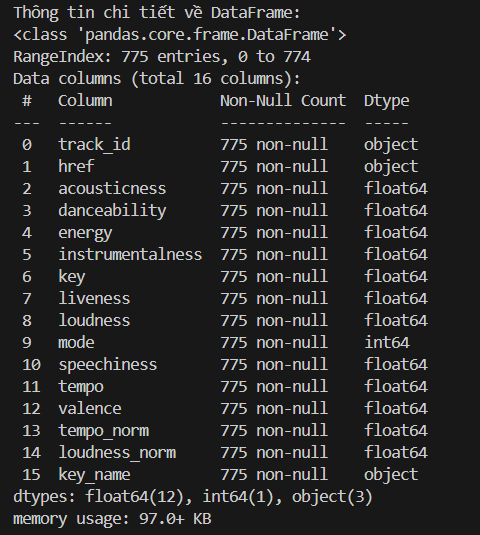
\includegraphics[width=0.75\textwidth]{../graphics/data_top50/figure/script/Screenshot 2025-10-02 192420.png} % tên file hình
    \caption{Đặc trưng chung} % chú thích
    \label{File meta-clean} % nhãn để tham chiếu
\end{figure}


\textbf{=> Kết quả:} ghi đè vào các file \texttt{...with-audio.csv} với các đặc trưng như trên.




\clearpage

















































\subsubsection{Phân tích và tìm insight:}
\begin{flushleft}
    

   
\textbf{-Công cụ khám phá: } Jupyter Notebook
\\

% \textbf{-Phân chia: } Do nguồn dataset khá lớn nên nhóm quyết định phân chia các bảng notebook thành các cụm đại diện thành các vùng dựa trên vị trí địa lý:
 
\end{flushleft}



% \begin{itemize}
%     \item \textbf{Châu Âu - Erope :} gồm italy, UK, france, spain
%     \item  \textbf{Châu Mỹ - America :} gồm argentina, usa , mexico
%     \item \textbf{Châu Á - Asia :} gồm south korea, japan
% \end{itemize}



\textbf{1. Bức tranh toàn diện về vòng đời âm nhạc trên BXH}
\begin{itemize}
    \item \textbf{1.1 Số bài hát mới phát hành theo năm}


    \begin{figure}[H]
        \centering
        % Dòng 1
        \begin{minipage}{0.45\textwidth}
            \centering
            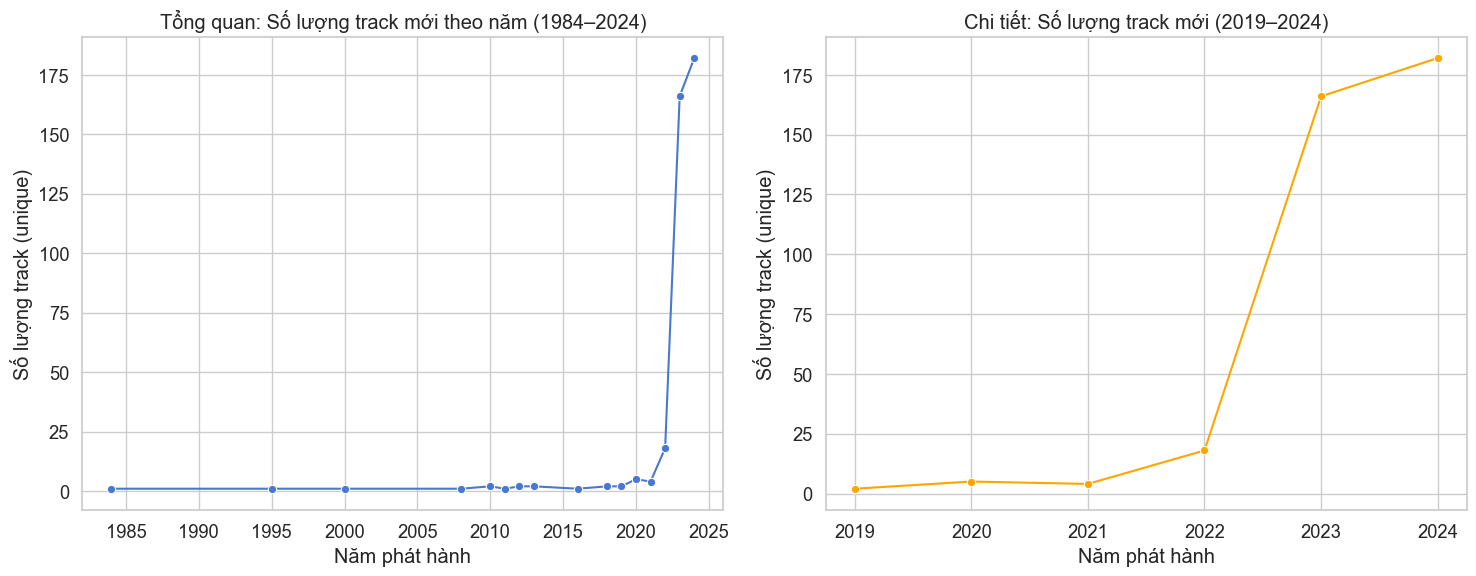
\includegraphics[width=\linewidth]{../graphics/data_top50/figure/10/EDA_argentina.png}
            \\[4pt] {\small \textbf{Argentina}}
        \end{minipage}
        \hfill
        \begin{minipage}{0.45\textwidth}
            \centering
            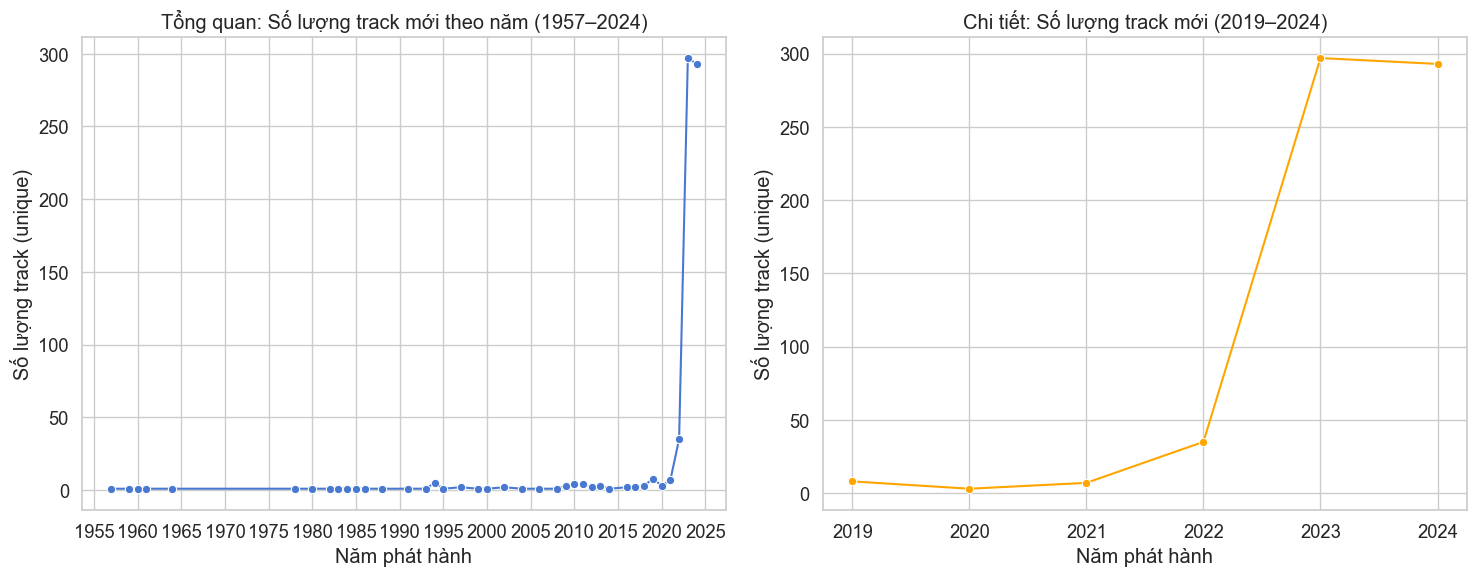
\includegraphics[width=\linewidth]{../graphics/data_top50/figure/10/EDA_france.png}
            \\[4pt] {\small \textbf{France}}
        \end{minipage}

        \vspace{0.4cm}

        % Dòng 2
        \begin{minipage}{0.45\textwidth}
            \centering
            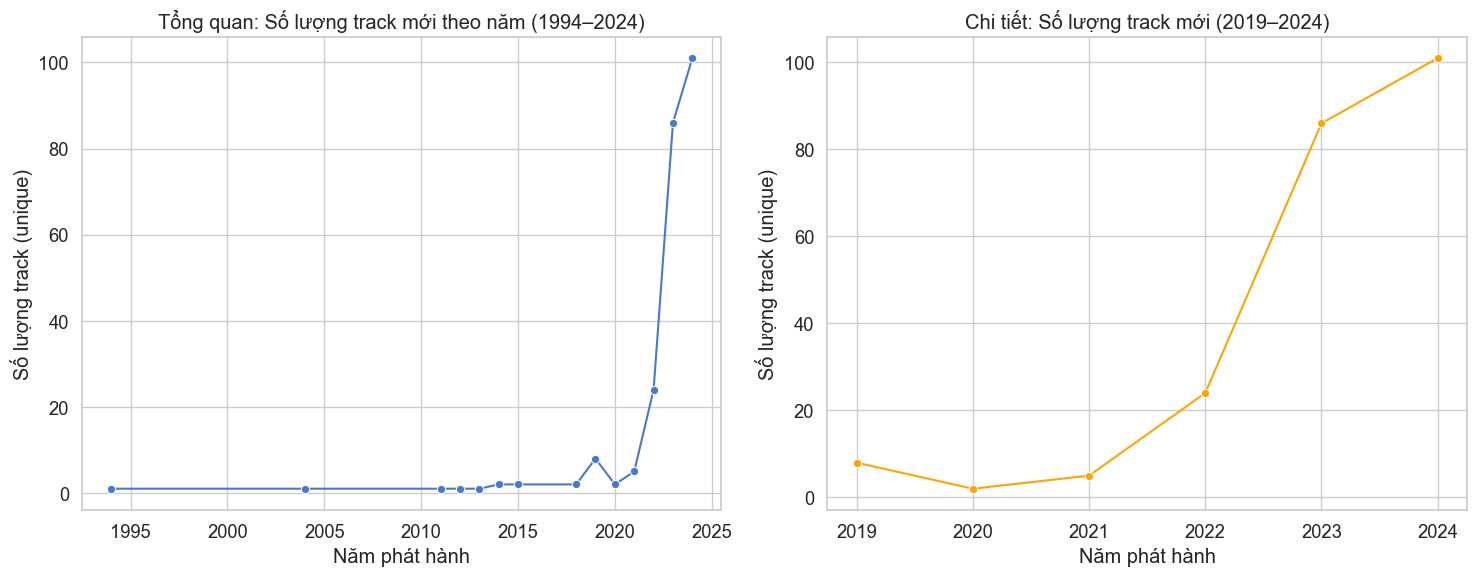
\includegraphics[width=\linewidth]{../graphics/data_top50/figure/10/EDA_japan.png}
            \\[4pt] {\small \textbf{Japan}}
        \end{minipage}
        \hfill
        \begin{minipage}{0.45\textwidth}
            \centering
            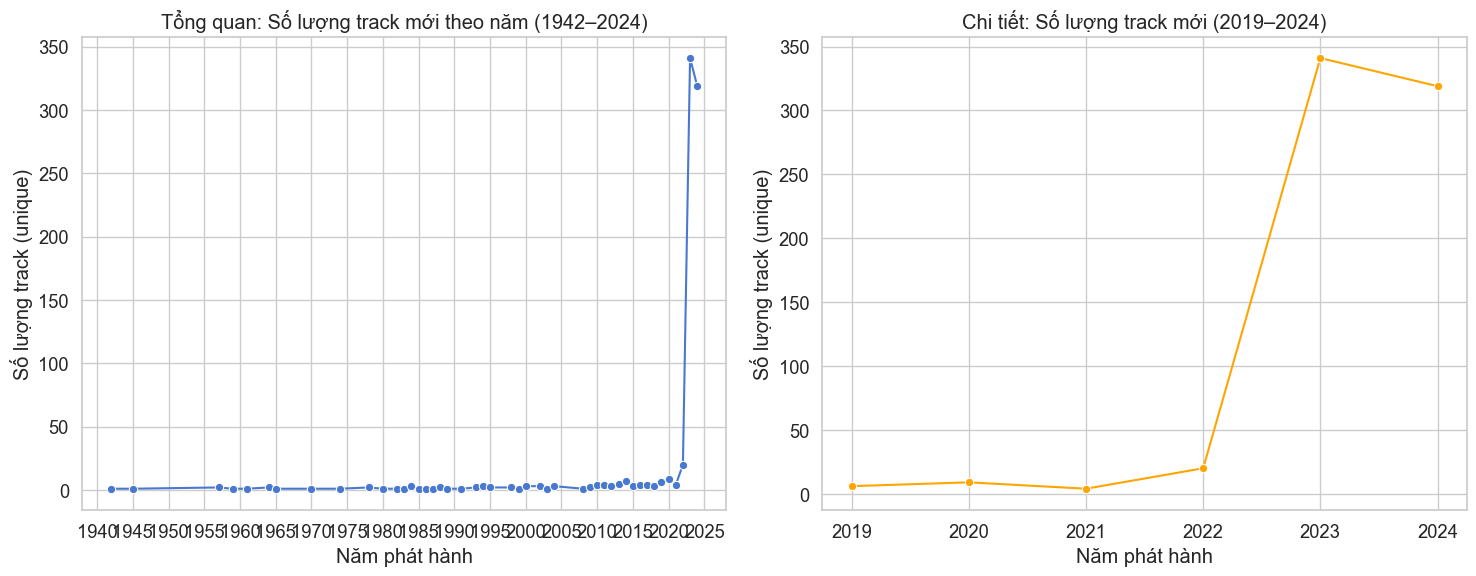
\includegraphics[width=\linewidth]{../graphics/data_top50/figure/10/EDA_world.png}
            \\[4pt] {\small \textbf{World}}
        \end{minipage}

        \caption{Track mới phát hành theo năm}
        \label{fig:energy-regions}
    \end{figure}
    
           \begin{itemize}
               \item \textbf{ Kết luận: }
               \item Trước năm 2015: số lượng track mới trên BXH rất ít, tăng trưởng chậm
               \item Giai đoạn 2015–2020: bắt đầu có xu hướng tăng nhưng chưa bùng nổ.
               \item Từ 2020 trở đi: số lượng track mới tăng vọt, đặc biệt 2023–2024 đạt đỉnh. Xuất hiện ở hầu hết quốc gia, mạnh nhất tại Mỹ \&\ Argentina, trong khi Hàn Quốc và Nhật Bản nổi bật nhờ K-pop và J-pop.
               \item Streaming và toàn cầu hoá đã tạo ra “làn sóng bùng nổ” sản xuất nhạc mới sau 2020
           \end{itemize}


    \item \textbf{1.2 Tuối thọ bài hát trên bảng xếp hạng:}



    \begin{figure}[H]
        \centering
        % Dòng 1
        \begin{minipage}{0.45\textwidth}
            \centering
            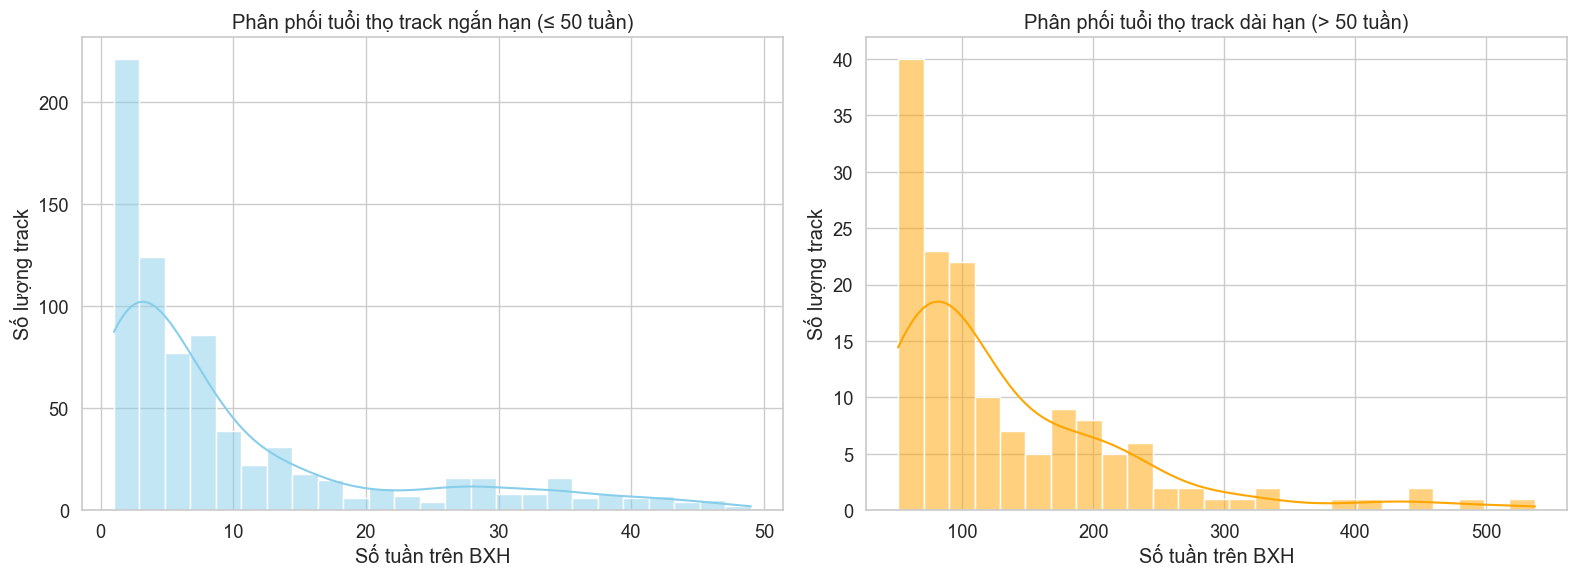
\includegraphics[width=\linewidth]{../graphics/data_top50/figure/11/EDA_usa.png}
            \\[4pt] {\small \textbf{USA}}
        \end{minipage}
        \hfill
        \begin{minipage}{0.45\textwidth}
            \centering
            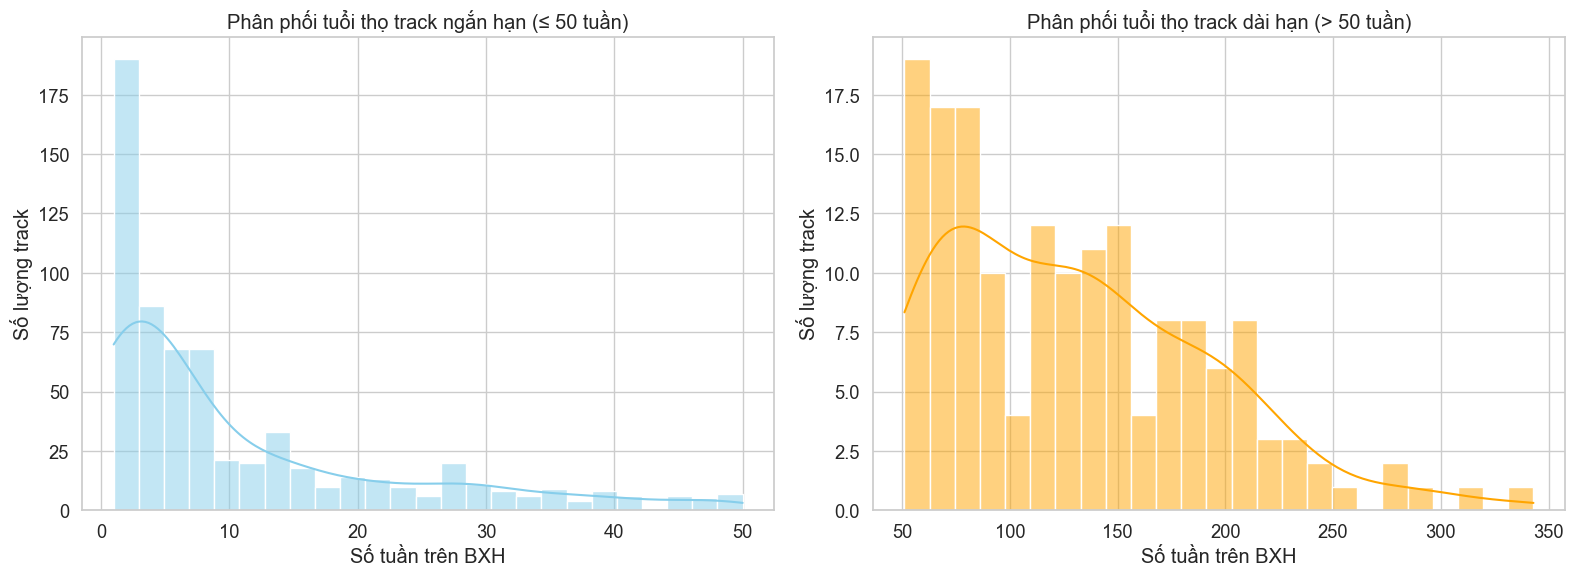
\includegraphics[width=\linewidth]{../graphics/data_top50/figure/11/EDA_italy.png}
            \\[4pt] {\small \textbf{Italy}}
        \end{minipage}

        \vspace{0.4cm}

        % Dòng 2
        \begin{minipage}{0.45\textwidth}
            \centering
            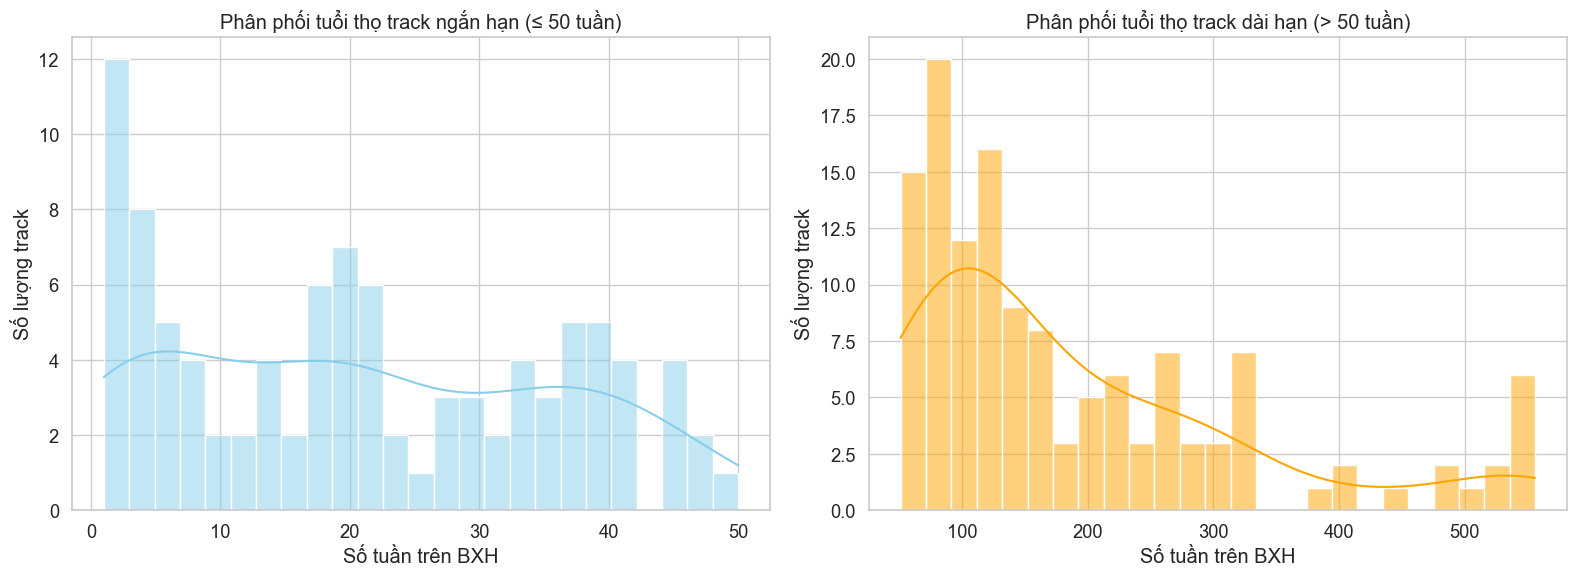
\includegraphics[width=\linewidth]{../graphics/data_top50/figure/11/EDA_japan.png}
            \\[4pt] {\small \textbf{Japan}}
        \end{minipage}
        \hfill
        \begin{minipage}{0.45\textwidth}
            \centering
            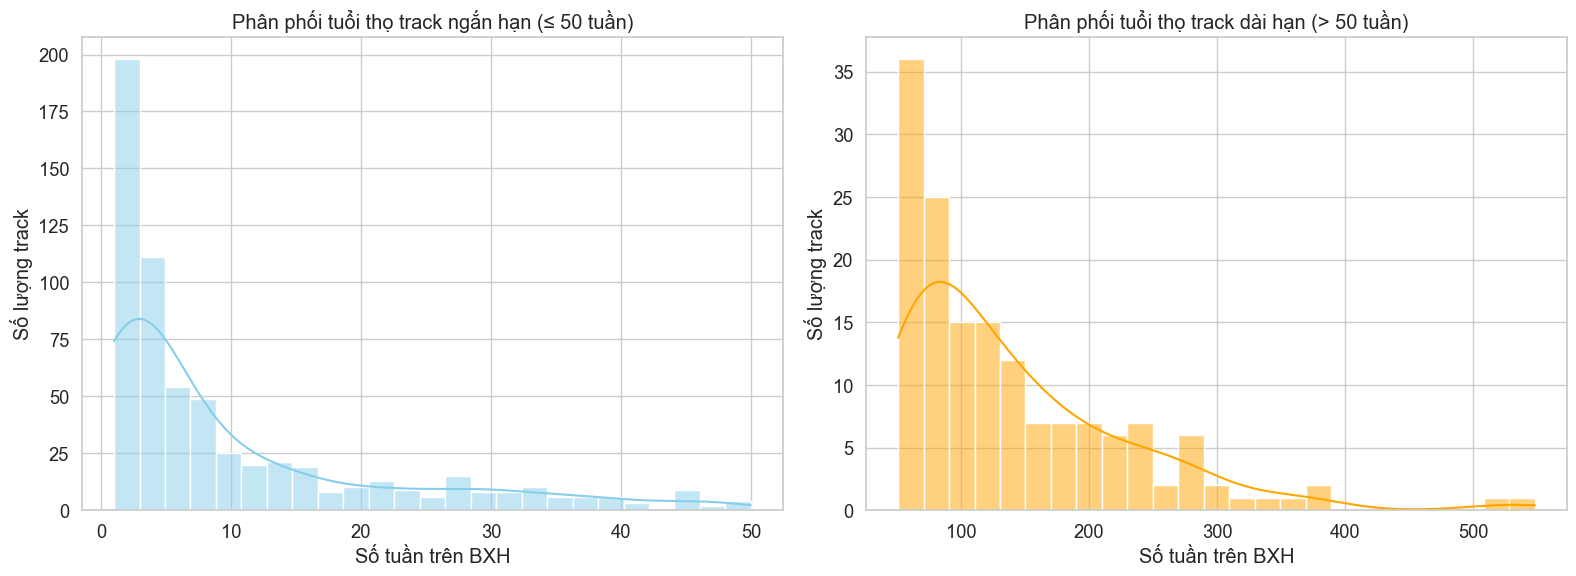
\includegraphics[width=\linewidth]{../graphics/data_top50/figure/11/EDA_world.png}
            \\[4pt] {\small \textbf{World}}
        \end{minipage}

        \caption{1.2 Tuổi thọ các bài hát trên BXH}
        \label{fig:energy-regions}
    \end{figure}


          \begin{itemize}
              \item \textbf{Kết luận: }
              \item Phần lớn bài hát có tuổi thọ ngắn, đa số bài hát chỉ trụ được dưới 10 tuần trên BXH => đặc trưng chung của BXH Top 50: hit bùng nổ nhanh nhưng cũng dễ rơi khỏi bảng.
              \item Vẫn tồn tại nhóm nhỏ có tuổi thọ dài (> 50 tuần), kéo dài đến 300–500 tuần.Những bài này thường là siêu hit toàn cầu hoặc gắn liền với văn hóa. 
              \item So sánh giữa các nước và thế giới: Ở cấp quốc gia, tuổi thọ thường ngắn hơn => thị trường có tính “nóng hổi”.Ở cấp thế giới, xuất hiện nhiều bài hát có tuổi thọ cực dài => tính bền vững và lan tỏa rộng.
              
          \end{itemize}

    \item\textbf{1.3 Độ biến động (volatility) trên BXH}


    \begin{figure}[H]
        \centering
        % Dòng 1
        \begin{minipage}{0.45\textwidth}
            \centering
            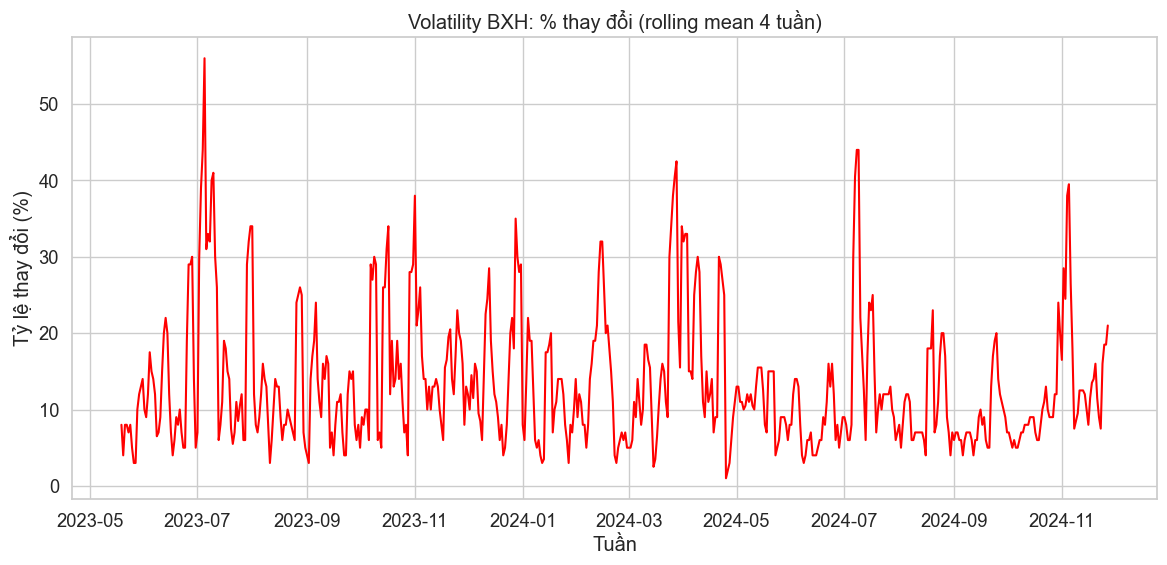
\includegraphics[width=\linewidth]{../graphics/data_top50/figure/12/EDA_usa.png}
            \\[4pt] {\small \textbf{USA}}
        \end{minipage}
        \hfill
        \begin{minipage}{0.45\textwidth}
            \centering
            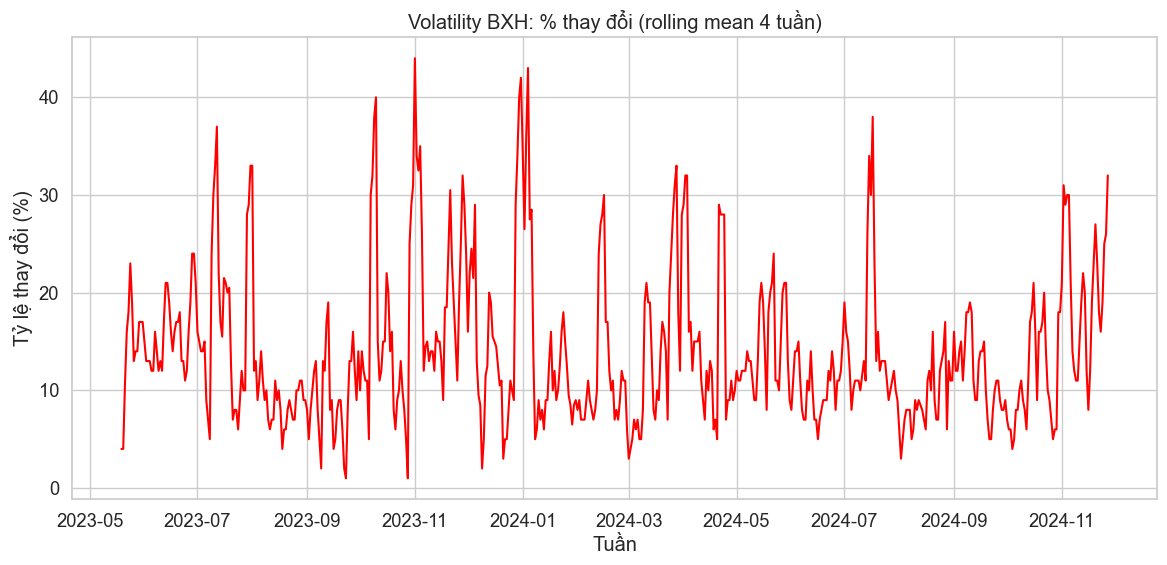
\includegraphics[width=\linewidth]{../graphics/data_top50/figure/12/EDA_uk.png}
            \\[4pt] {\small \textbf{UK}}
        \end{minipage}

        \vspace{0.4cm}

        % Dòng 2
        \begin{minipage}{0.45\textwidth}
            \centering
            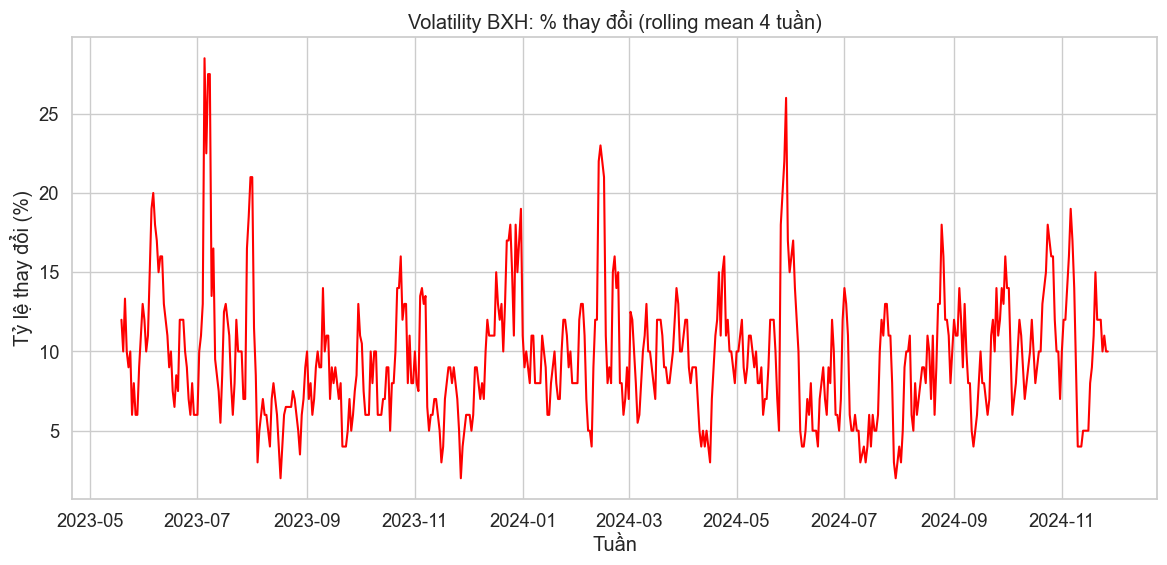
\includegraphics[width=\linewidth]{../graphics/data_top50/figure/12/EDA_south_korea.png}
            \\[4pt] {\small \textbf{Korea}}
        \end{minipage}
        \hfill
        \begin{minipage}{0.45\textwidth}
            \centering
            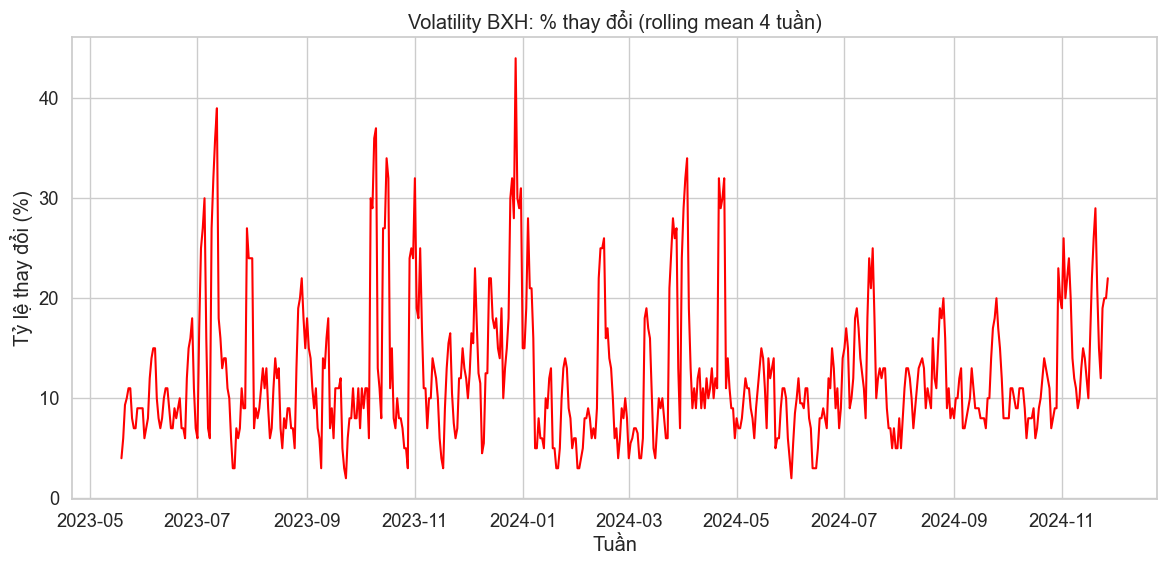
\includegraphics[width=\linewidth]{../graphics/data_top50/figure/12/EDA_world.png}
            \\[4pt] {\small \textbf{World}}
        \end{minipage}



        % Dòng 3
        \begin{minipage}{0.45\textwidth}
            \centering
            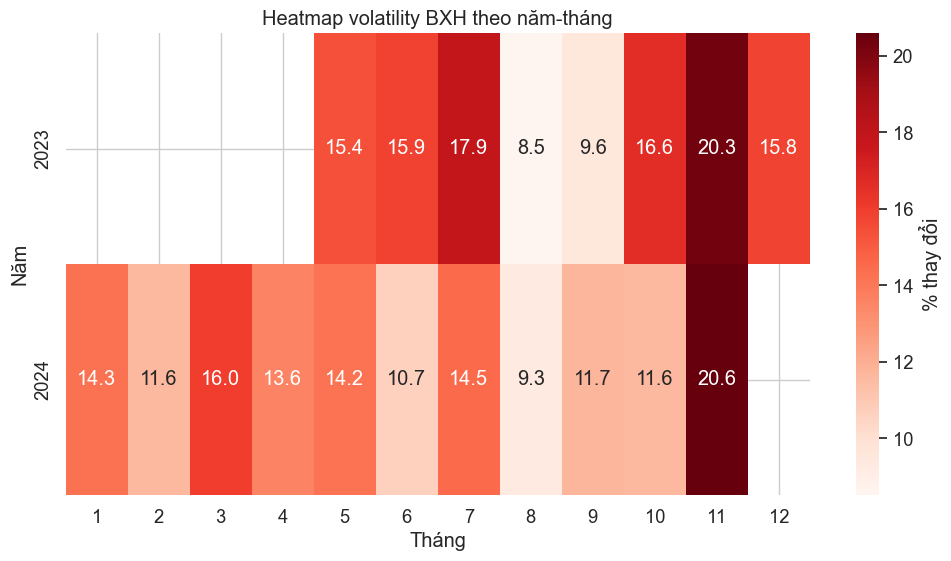
\includegraphics[width=\linewidth]{../graphics/data_top50/figure/14/EDA_uk.png}
            \\[4pt] {\small \textbf{UK}}
        \end{minipage}
        \hfill
        \begin{minipage}{0.45\textwidth}
            \centering
            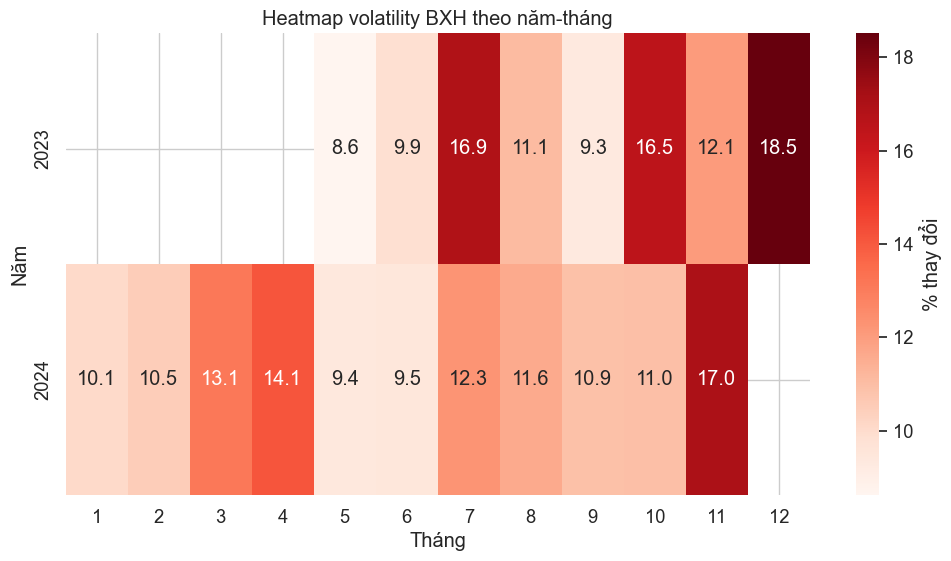
\includegraphics[width=\linewidth]{../graphics/data_top50/figure/14/EDA_world.png}
            \\[4pt] {\small \textbf{World}}
        \end{minipage}

        \caption{1.2 Độ biến động tổng quan trên BXH}
        \label{fig:energy-regions}

        
    \end{figure}



        \begin{itemize}
            \item \textbf{Kết luận: }
            \item Mức biến động cao ở nhiều thị trường lớn, Mỹ, Anh thường có volatility > 20–30\%\ trong nhiều giai đoạn. Cho thấy cạnh tranh gay gắt, các ca khúc nhanh chóng leo hạng và rời BXH
            \item Một số thị trường ổn định hơn Nhật, Ý, Tây Ban Nha có volatility thấp hơn (chủ yếu < 15\%\ ). Điều này phản ánh thị hiếu nghe nhạc ổn định, ít thay đổi đột ngột theo xu hướng.
            \item Đặc thù mùa vụ và sự kiện âm nhạc:
             Các đỉnh biến động thường rơi vào dịp cuối năm, mùa lễ hội.
               Ví dụ: giai đoạn cuối 2023 và giữa 2024 có nhiều peak volatility (đỉnh) đồng loạt ở nhiều nước.
        \end{itemize}

    

          
\end{itemize}


\textbf{2. Nghệ sĩ và Bài hát}

\begin{itemize}

    \item \textbf{2.1 Top 10 nghệ sĩ phổ biến}



    \begin{figure}[H]
        \centering
        % Dòng 1
        \begin{minipage}{0.45\textwidth}
            \centering
            \includegraphics[width=\linewidth]{../graphics/data_top50/figure/0/EDA_USA.png}
            \\[4pt] {\small \textbf{USA}}
        \end{minipage}
        \hfill
        \begin{minipage}{0.45\textwidth}
            \centering
            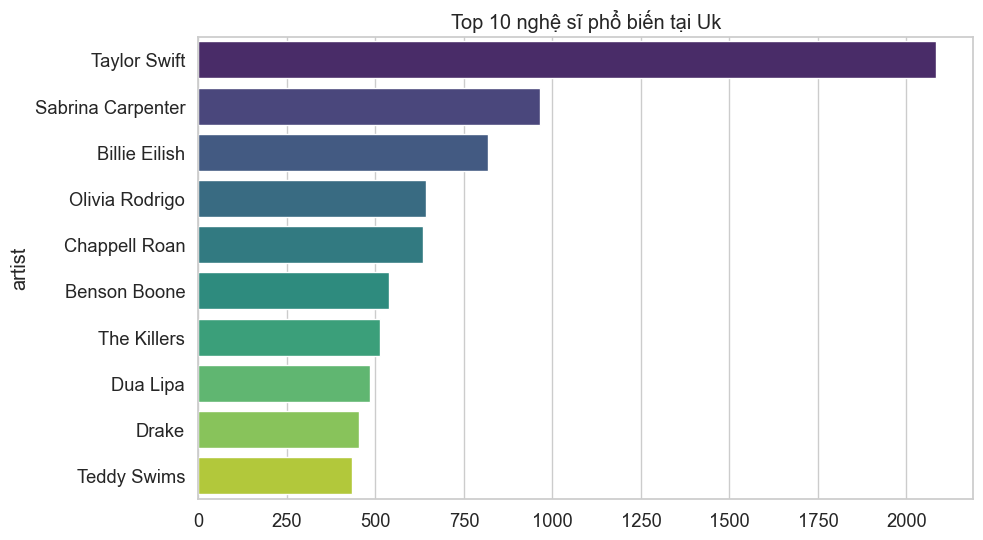
\includegraphics[width=\linewidth]{../graphics/data_top50/figure/0/EDA_uk.png}
            \\[4pt] {\small \textbf{UK}}
        \end{minipage}

        \vspace{0.4cm}

        % Dòng 2
        \begin{minipage}{0.45\textwidth}
            \centering
            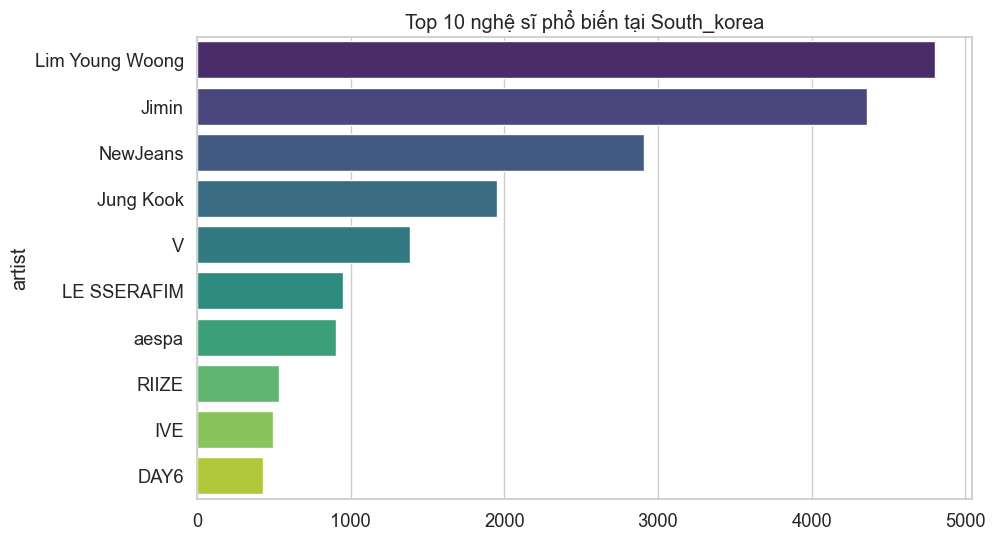
\includegraphics[width=\linewidth]{../graphics/data_top50/figure/0/EDA_south_korea.png}
            \\[4pt] {\small \textbf{Korea}}
        \end{minipage}
        \hfill
        \begin{minipage}{0.45\textwidth}
            \centering
            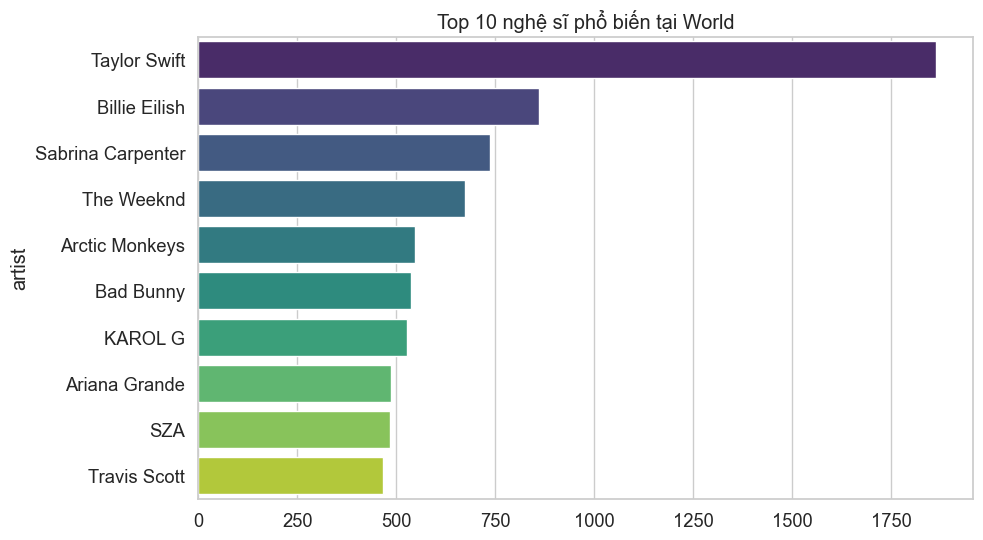
\includegraphics[width=\linewidth]{../graphics/data_top50/figure/0/EDA_world.png}
            \\[4pt] {\small \textbf{World}}
        \end{minipage}



        
        \caption{Top 10 nghệ sĩ nổi bật nhất}
        \label{fig:energy-regions}
    \end{figure}
    
        \begin{itemize}
            \item \textbf{Kết luận: }
            \item Nhìn chung đa số quốc gia có nghệ sĩ nội địa thống trị: ví dụ Emilia, Luck Ra (Argentina), Werenoi (France), Geolier, Tedua (Italy), Mrs. GREEN APPLE, YOASOBI (Japan), Peso Pluma (Mexico), Lim Young Woong, BTS members, NewJeans (Korea).
            \item Riêng thị trường Âu–Mỹ vẫn nổi bật với những ngôi sao toàn cầu: Taylor Swift, Billie Eilish, Drake, Bad Bunny, KAROL G… thường xuyên góp mặt cả ở BXH quốc gia và World.
            \item Có sự khác biệt rõ rệt giữa thị hiếu nội địa và toàn cầu: Nhật, Hàn Quốc chủ yếu nghệ sĩ bản địa; trong khi BXH World và Mỹ/UK có nhiều nghệ sĩ đa quốc gia.
        \end{itemize}







    \item \textbf{2.2 Bài hát theo độ hot}



    \begin{figure}[H]
        \centering
        % Dòng 1
        \begin{minipage}{0.4\textwidth}
            \centering
            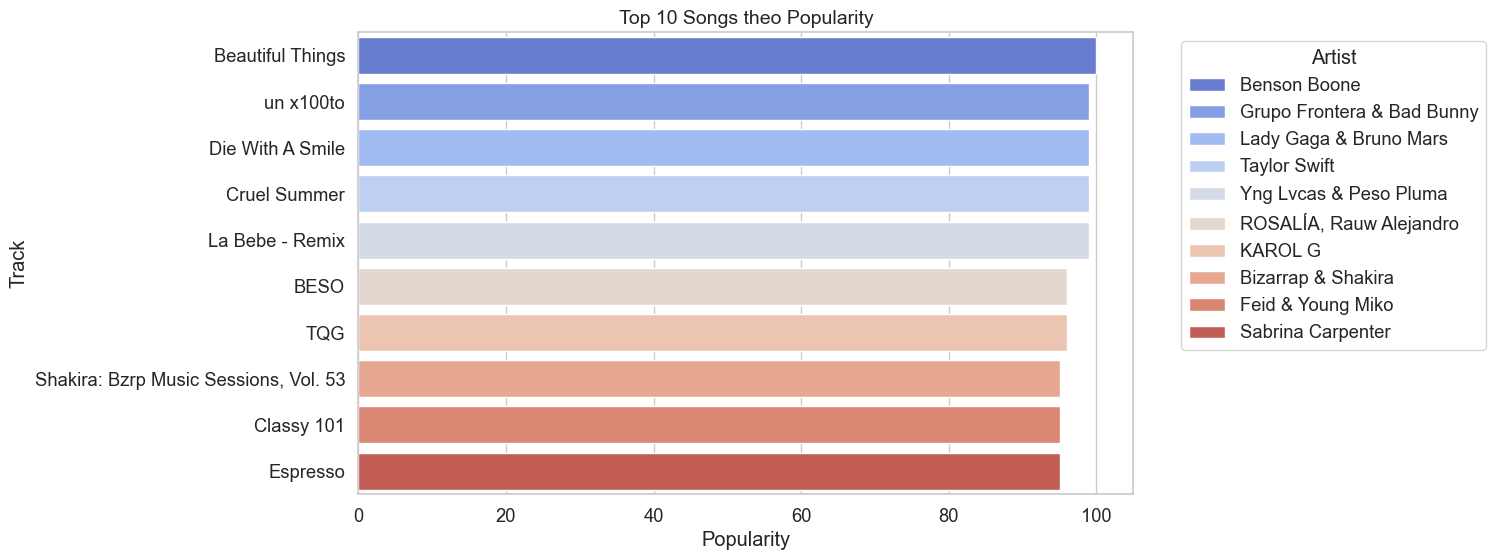
\includegraphics[width=\linewidth]{../graphics/data_top50/figure/2/EDA_argentina.png}
            \\[4pt] {\small \textbf{Argentina}}
        \end{minipage}
        \hfill
        \begin{minipage}{0.4\textwidth}
            \centering
            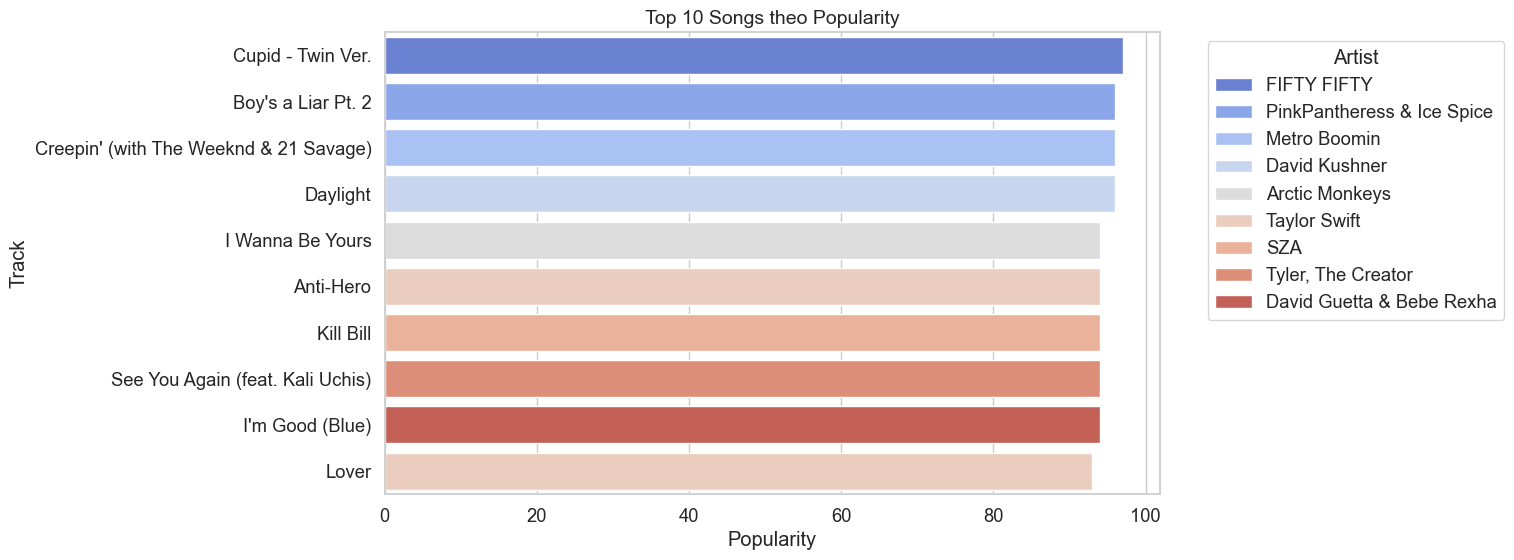
\includegraphics[width=\linewidth]{../graphics/data_top50/figure/2/EDA_uk.png}
            \\[4pt] {\small \textbf{UK}}
        \end{minipage}

        \vspace{0.4cm}

        % Dòng 2
        \begin{minipage}{0.4\textwidth}
            \centering
            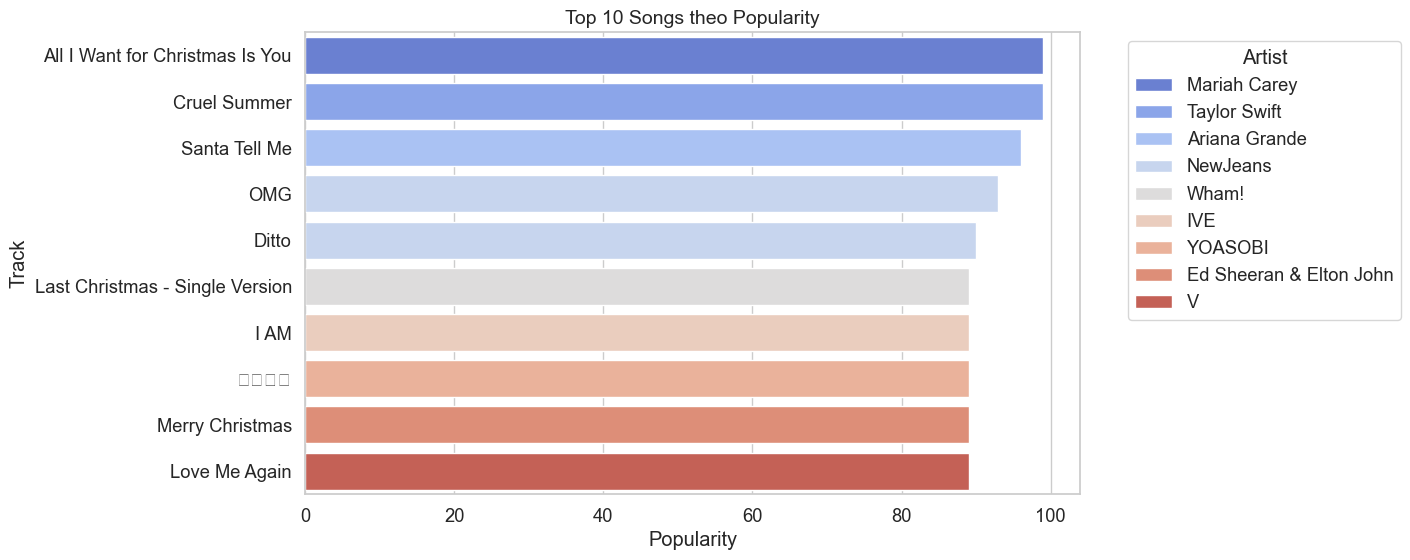
\includegraphics[width=\linewidth]{../graphics/data_top50/figure/2/EDA_japan.png}
            \\[4pt] {\small \textbf{Japan}}
        \end{minipage}
        \hfill
        \begin{minipage}{0.4\textwidth}
            \centering
            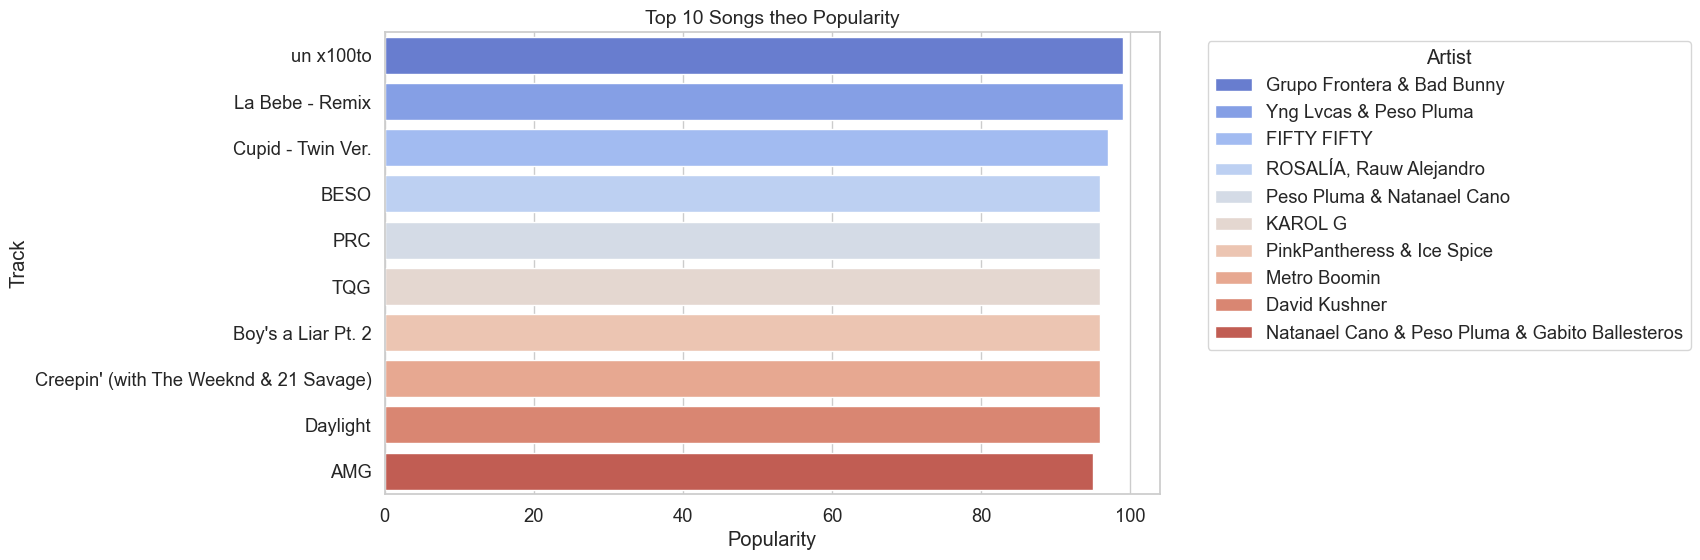
\includegraphics[width=\linewidth]{../graphics/data_top50/figure/2/EDA_world.png}
            \\[4pt] {\small \textbf{World}}
        \end{minipage}
        
        \caption{Top 10 bài hát trụ nổi nhất}
        \label{fig:energy-regions}

        \vspace{0.4cm}
        \begin{minipage}{1\textwidth}
            \centering
            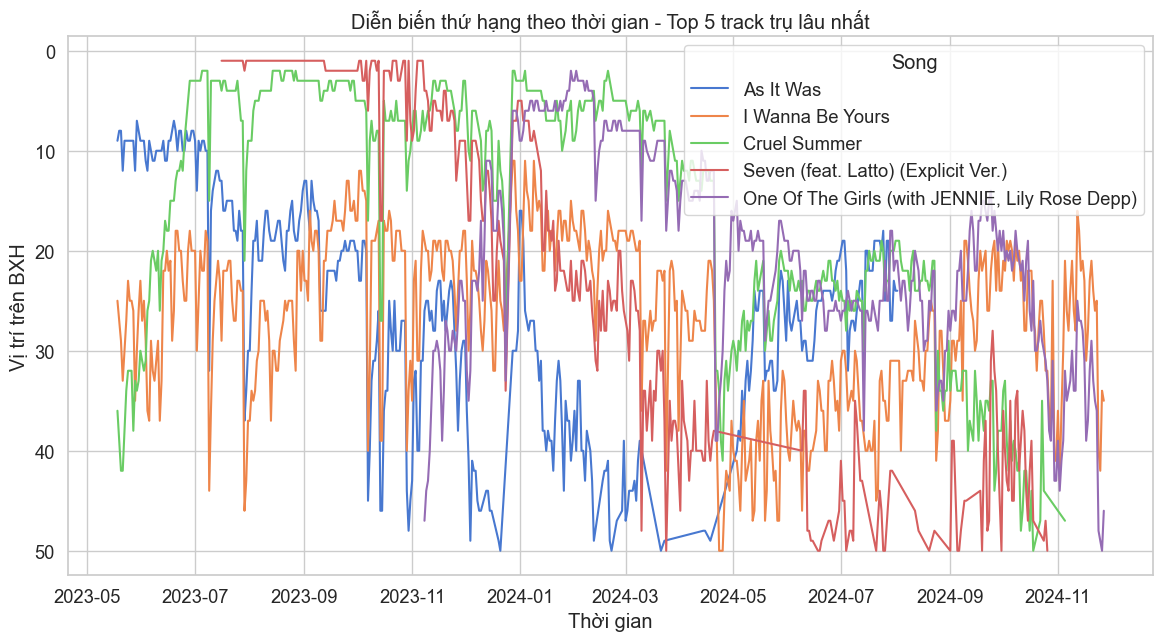
\includegraphics[width=\linewidth]{../graphics/data_top50/figure/17/EDA_world.png}
            \\[4pt] {\small \textbf{World}}
        \end{minipage}
        
        \caption{Top 5 bài hát trụ lâu nhất}
         \label{fig:energy-regions}

     \end{figure}

                % Dòng 2
        


      
    
   

         \begin{itemize}
             \item \textbf{Kết luận: }
             \item Top 10 bài hát phổ biến: mỗi quốc gia có “quốc ca nội địa” riêng , trong khi BXH World lại nổi bật với các siêu hit toàn cầu .
             
             \item  Top 5 bài hát trụ lâu nhất : Cho thấy sự khác biệt giữa các thị trường: US/UK có những bản hit lâu bền, Hàn Quốc ghi dấu với loạt K-pop nổi bật, còn các nước Mỹ Latin có nhiều ca khúc trụ lâu thuộc dòng nhạc địa phương. Trên BXH World, một số siêu hit quốc tế  thể hiện sức hút bền vững, duy trì thứ hạng cao trong nhiều tháng.

             
             \item So sánh quốc gia – thế giới cho thấy: bài hát nội địa thường nổi trong nước nhưng ít khi bền vững toàn cầu, ngược lại siêu hit quốc tế có sức lan tỏa rộng và trụ lâu hơn

             
         \end{itemize}
\end{itemize}




\textbf{3. Thể loại}
\begin{itemize}
    \item \textbf{3.1 Top 10 thể loại phổ biến}


    \begin{figure}[H]
        \centering
        % Dòng 1
        \begin{minipage}{0.35\textwidth}
            \centering
            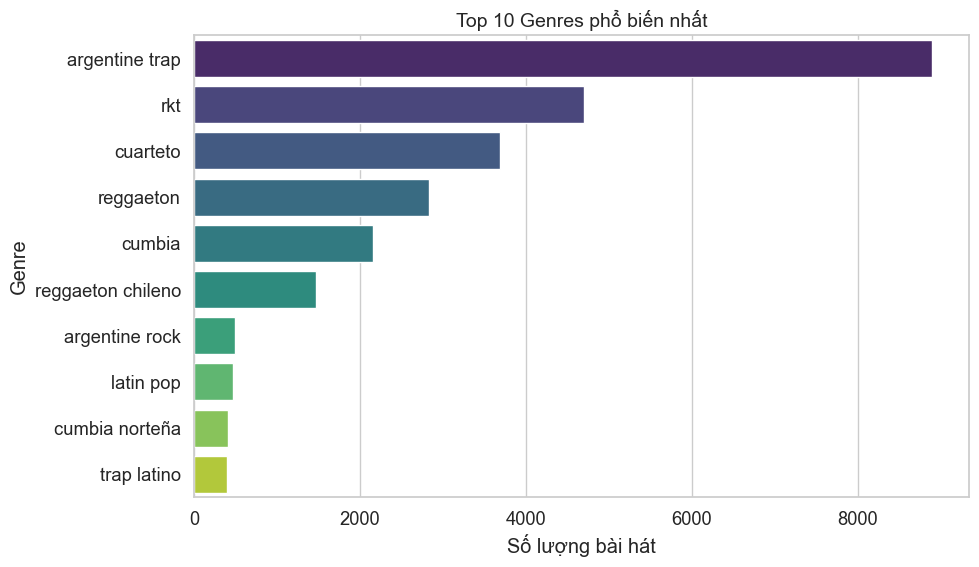
\includegraphics[width=\linewidth]{../graphics/data_top50/figure/1/EDA_argentina.png}
            \\[4pt] {\small \textbf{Argentina}}
        \end{minipage}
        \hfill
        \begin{minipage}{0.35\textwidth}
            \centering
            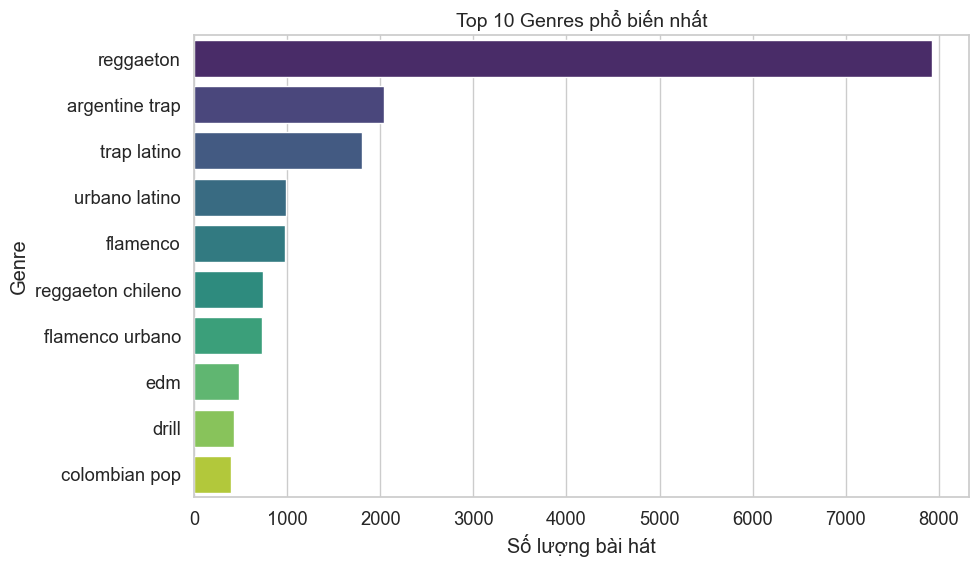
\includegraphics[width=\linewidth]{../graphics/data_top50/figure/1/EDA_spain.png}
            \\[4pt] {\small \textbf{Spain}}
        \end{minipage}

        \vspace{0.4cm}

        % Dòng 2
        \begin{minipage}{0.35\textwidth}
            \centering
            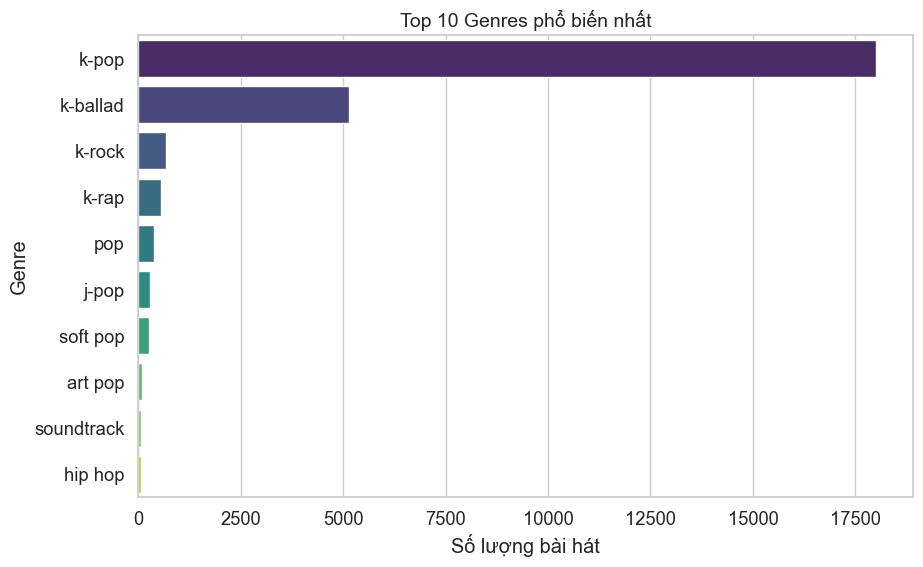
\includegraphics[width=\linewidth]{../graphics/data_top50/figure/1/EDA_south_korea.png}
            \\[4pt] {\small \textbf{Korea}}
        \end{minipage}
        \hfill
        \begin{minipage}{0.35\textwidth}
            \centering
            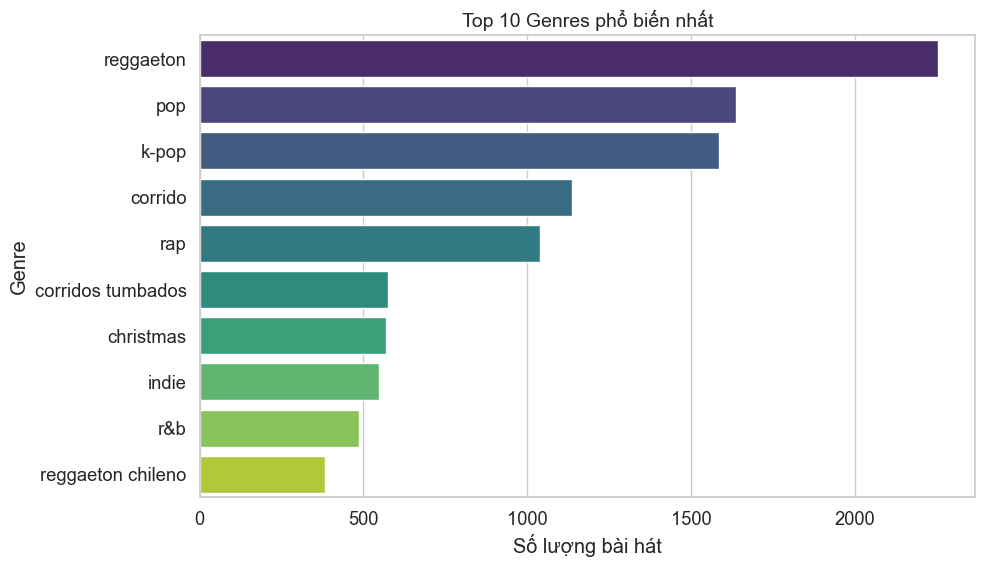
\includegraphics[width=\linewidth]{../graphics/data_top50/figure/1/EDA_world.png}
            \\[4pt] {\small \textbf{World}}
        \end{minipage}



        
        \caption{Top 10 thể loại nổi bật nhất}
        \label{fig:energy-regions}
    \end{figure}
    

    
    \begin{itemize}
        \item \textbf{Kết luận: }
        \item Mỗi quốc gia có thể loại bản địa thống trị, ví dụ:Argentina (Argentine trap, RKT, cuarteto), Japan (J-pop, Anime, J-rock), ..
        
        % \begin{itemize}
        %     \item Argentina => Argentine trap, RKT, cuarteto

        %      \item France => French rap, French R \&\ B

        %         \item Italy => Italian trap, Canzone napoletana

        %         \item Japan => J-pop, Anime, J-rock

        %        \item Mexico => Corrido, Corridos tumbados, Banda

        %       \item Korea => K-pop, K-ballad

        %    \item Spain => Reggaeton, Flamenco

        %      \item US/UK => Pop, Rap, Country, Alternative rock.
        % \end{itemize}

        \item Sự khác biệt văn hoá rõ rệt: Nhật – Hàn nghiêng về nhạc bản địa (J-pop, K-pop), Mexico – LATAM mạnh về reggaeton/corrido, còn Âu–Mỹ giữ vị thế với pop/rap.
        \item Xu hướng toàn cầu: Một số thể loại vượt biên giới mạnh mẽ (reggaeton, trap, pop, rap) => lan toả sang nhiều thị trường khác nhau.
    \end{itemize}

   \item \textbf{3.1 Xu hướng thể loại theo thời gian}


   
    \begin{figure}[H]
        \centering
        % Dòng 1
        \begin{minipage}{0.45\textwidth}
            \centering
            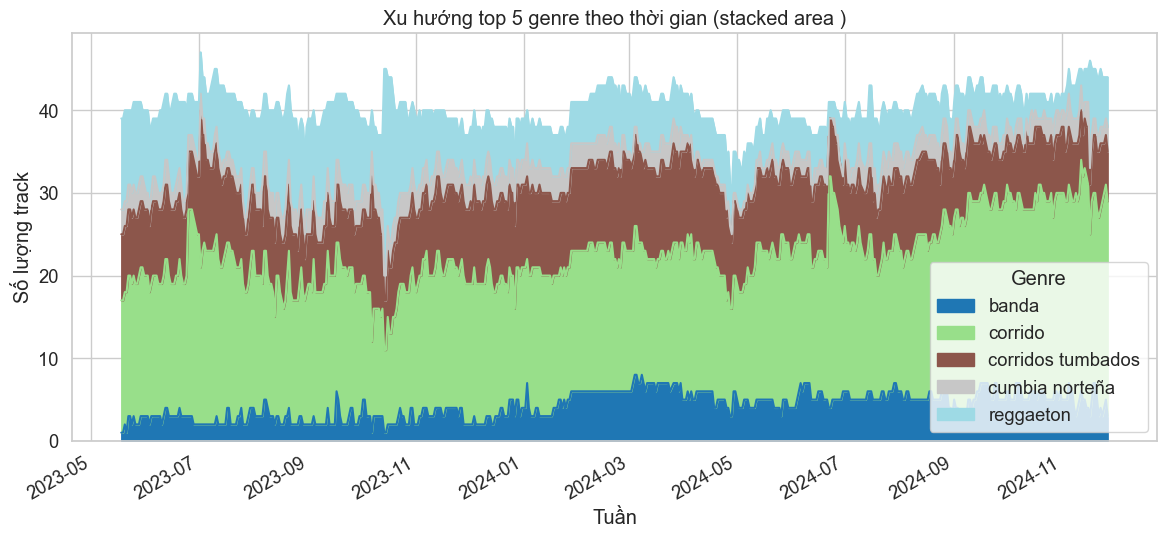
\includegraphics[width=\linewidth]{../graphics/data_top50/figure/25/EDA_mexico.png}
            \\[4pt] {\small \textbf{Mexico}}
        \end{minipage}
        \hfill
        \begin{minipage}{0.45\textwidth}
            \centering
            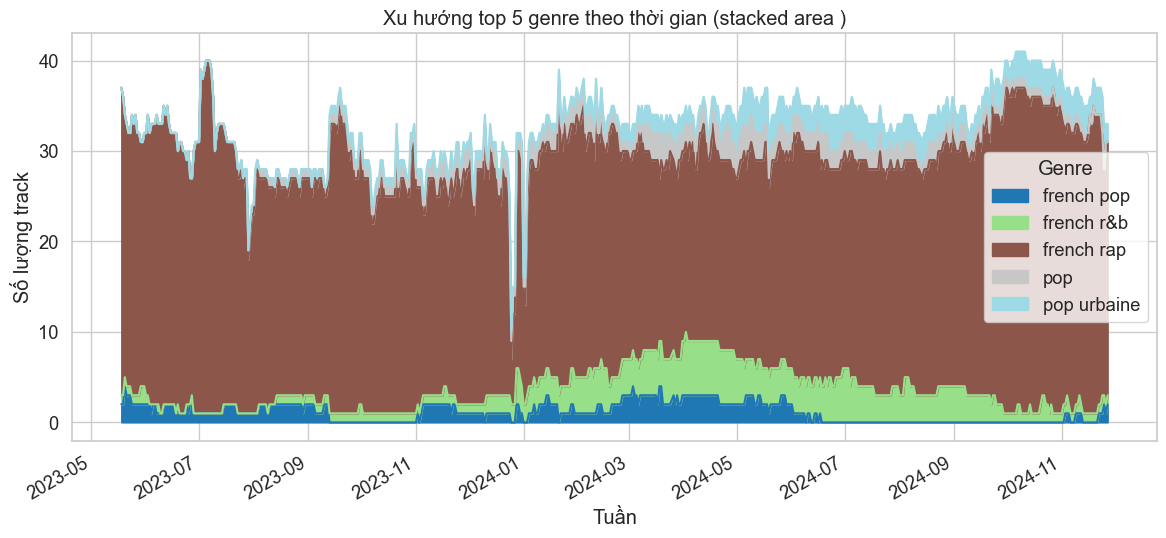
\includegraphics[width=\linewidth]{../graphics/data_top50/figure/25/EDA_france.png}
            \\[4pt] {\small \textbf{France}}
        \end{minipage}

        \vspace{0.4cm}

        % Dòng 2
        \begin{minipage}{0.45\textwidth}
            \centering
            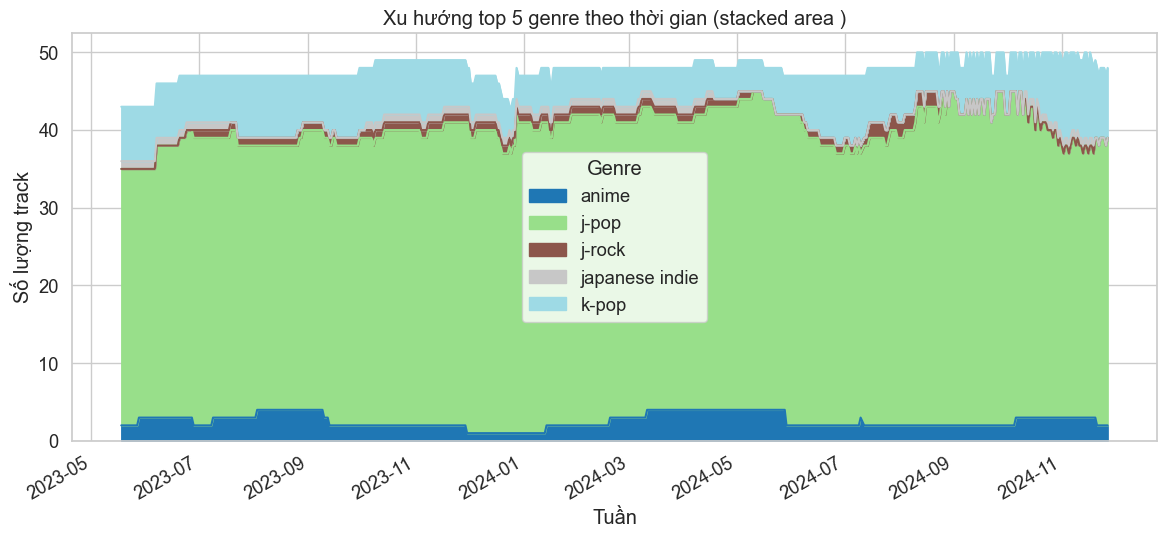
\includegraphics[width=\linewidth]{../graphics/data_top50/figure/25/EDA_japan.png}
            \\[4pt] {\small \textbf{Japan}}
        \end{minipage}
        \hfill
        \begin{minipage}{0.45\textwidth}
            \centering
            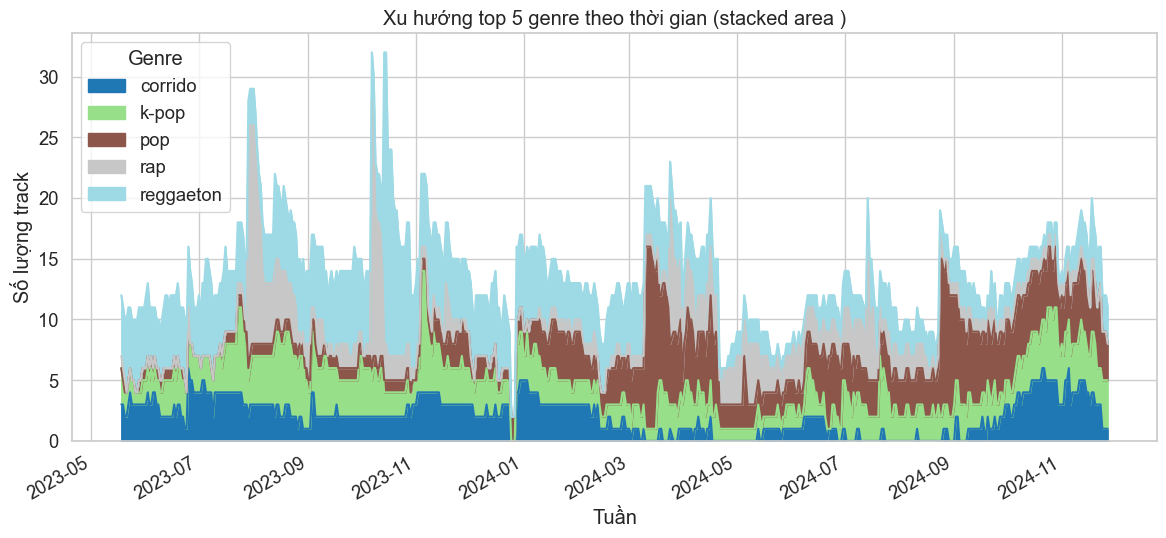
\includegraphics[width=\linewidth]{../graphics/data_top50/figure/25/EDA_world.png}
            \\[4pt] {\small \textbf{World}}
        \end{minipage}

        \caption{Top 10 thể loại nổi bật nhất}
    \end{figure}

    \begin{itemize}
        \item \textbf{Kết luận:}
        \item Genre bản địa áp đảo ổn định: J-pop (Japan), K-pop/K-ballad (Korea), French rap (France), Italian trap (Italy).
        \item Đa dạng nhất: Mexico – sự kết hợp của corrido, banda, tumbados, reggaeton, cumbia norteña.

        \item Khép kín: Nhật và Hàn hầu như chỉ nghe nhạc nội địa.
        \item Thể loại Latin (reggaeton, corrido, trap latino) tăng mạnh tại Argentina, Mexico, Spain và có sức lan tỏa sang thị trường quốc tế.
        \item Thể loại mùa vụ như Christmas nổi bật ở US/UK, tạo các đỉnh ngắn hạn cuối năm.

        \item Thị trường toàn cầu (World) cho thấy sự kết hợp của reggaeton, K-pop và pop/rap, phản ánh sự giao thoa văn hoá âm nhạc xuyên biên giới.
    \end{itemize}

    \begin{figure}[H]
        \centering
        % Dòng 1
        \begin{minipage}{0.45\textwidth}
            \centering
            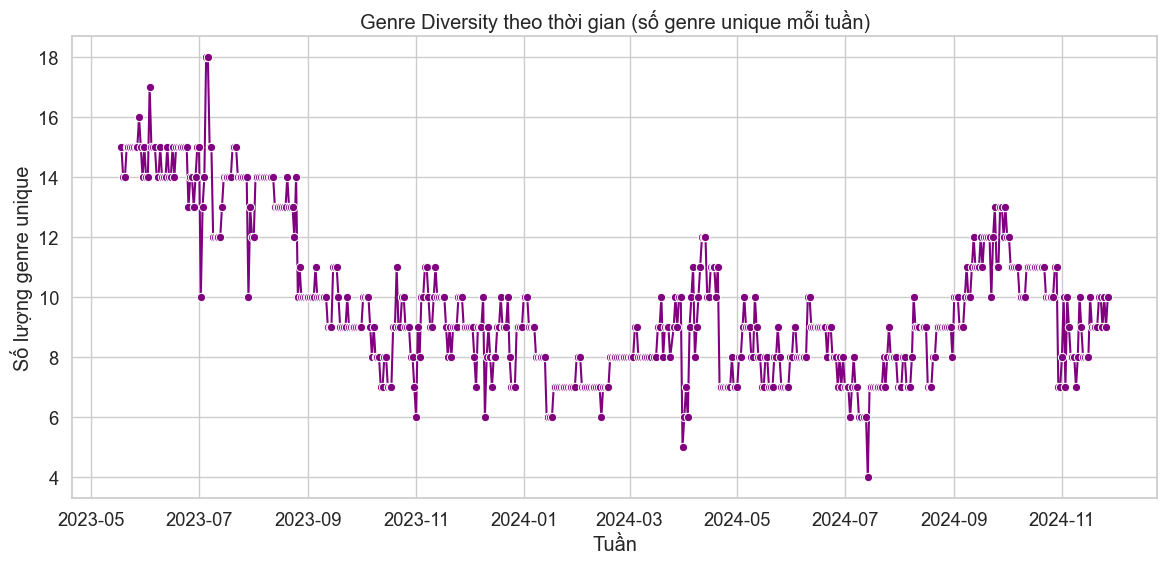
\includegraphics[width=\linewidth]{../graphics/data_top50/figure/24/EDA_usa.png}
            \\[4pt] {\small \textbf{USA}}
        \end{minipage}
        \hfill
        \begin{minipage}{0.45\textwidth}
            \centering
            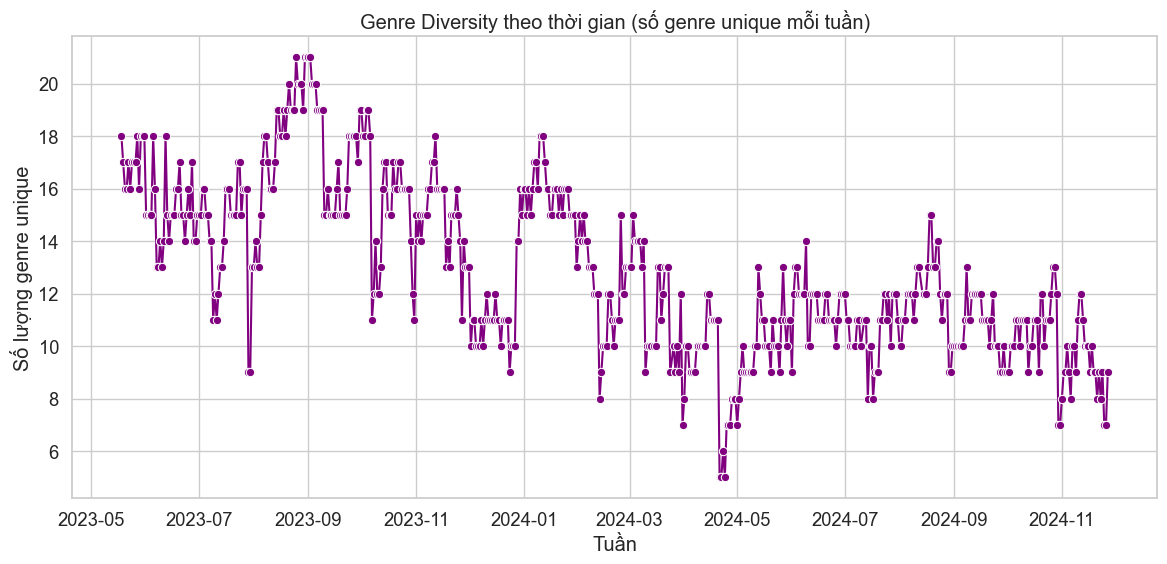
\includegraphics[width=\linewidth]{../graphics/data_top50/figure/24/EDA_uk.png}
            \\[4pt] {\small \textbf{UK}}
        \end{minipage}

        \vspace{0.4cm}

        % Dòng 2
        \begin{minipage}{0.45\textwidth}
            \centering
            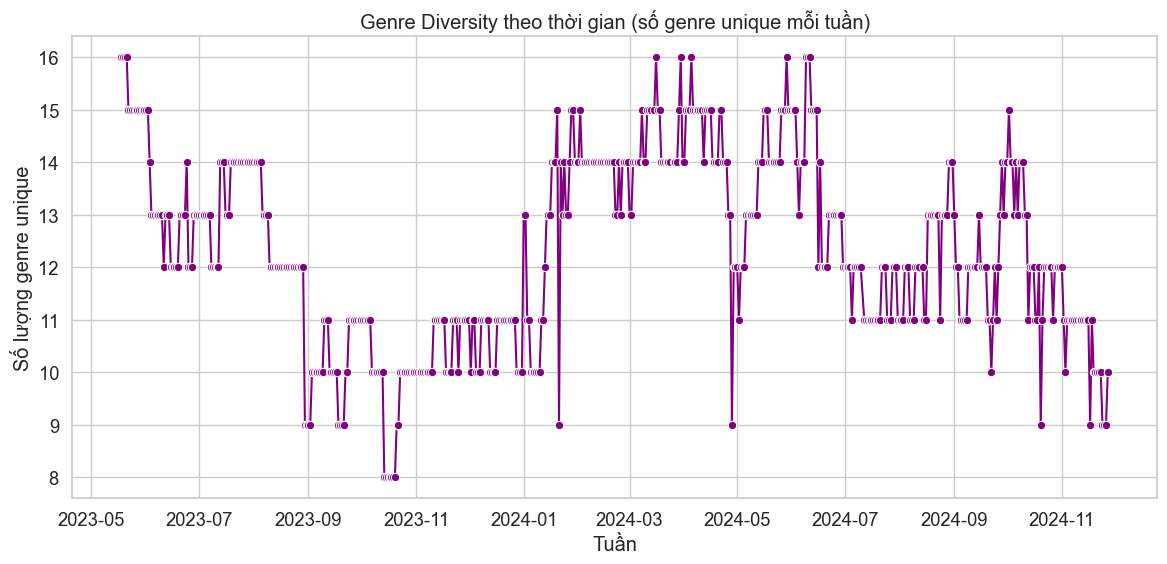
\includegraphics[width=\linewidth]{../graphics/data_top50/figure/24/EDA_spain.png}
            \\[4pt] {\small \textbf{Spain}}
        \end{minipage}
        \hfill
        \begin{minipage}{0.45\textwidth}
            \centering
            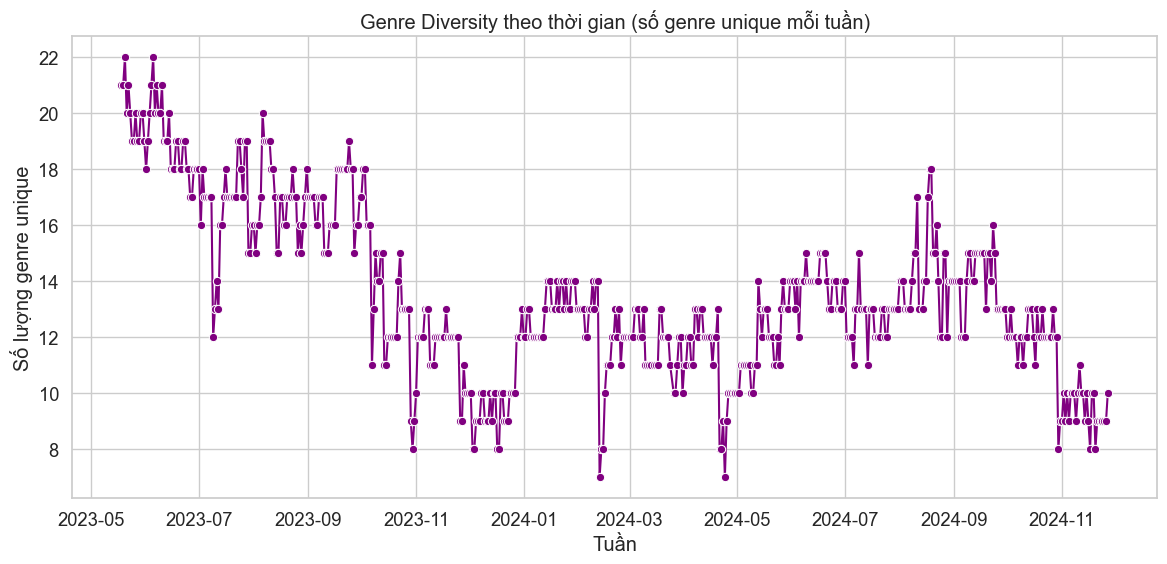
\includegraphics[width=\linewidth]{../graphics/data_top50/figure/24/EDA_world.png}
            \\[4pt] {\small \textbf{World}}
        \end{minipage}



        



        
        \caption{Độ đa dạng theo tuần}
    \end{figure}


    \begin{itemize}
        \item \textbf{Kết luận: }
        \item Khác biệt thị trường: US và World đa dạng nhất (10–22 genre/tuần), trong khi Nhật, Hàn, Ý khá tập trung (5–12 genre, chủ yếu J-pop, K-pop, Italian trap).

        \item Xu hướng mùa vụ: US/UK xuất hiện nhiều genre phụ cuối năm (Christmas, country, grime), còn Nhật/Hàn ổn định quanh 5–8 genre.

        \item Mỹ Latin (Argentina, Mexico, Spain): trung bình 8–15 genre, xoay quanh reggaeton, corrido, trap latino => ít bùng nổ thể loại mới.
        \item  Nhật Bản \&\ Hàn Quốc: số genre unique thấp và ổn định (5–8/tuần), gần như bị áp đảo bởi J-pop (Japan) và K-pop/K-ballad (Korea).
    \end{itemize}
\end{itemize}


 


\textbf{4. Đặc trưng âm nhạc}
\begin{itemize}
    \item \textbf{4.1 Đặc trưng energy}
    \begin{itemize}


   \begin{figure}[H]
        \centering
        % Dòng 1
        \begin{minipage}{0.45\textwidth}
            \centering
            \includegraphics[width=\linewidth]{../graphics/data_top50/figure/3/EDA_USA.png}
            \\[4pt] {\small \textbf{USA}}
        \end{minipage}
        \hfill
        \begin{minipage}{0.45\textwidth}
            \centering
            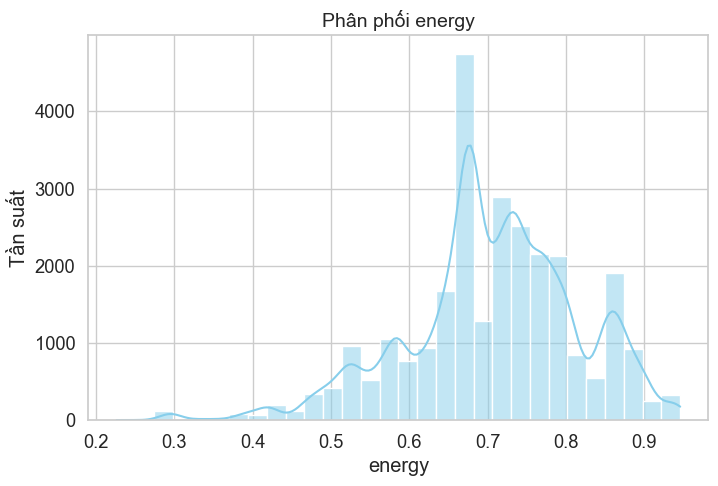
\includegraphics[width=\linewidth]{../graphics/data_top50/figure/3/EDA_spain.png}
            \\[4pt] {\small \textbf{Spain}}
        \end{minipage}

        \vspace{0.4cm}

        % Dòng 2
        \begin{minipage}{0.45\textwidth}
            \centering
            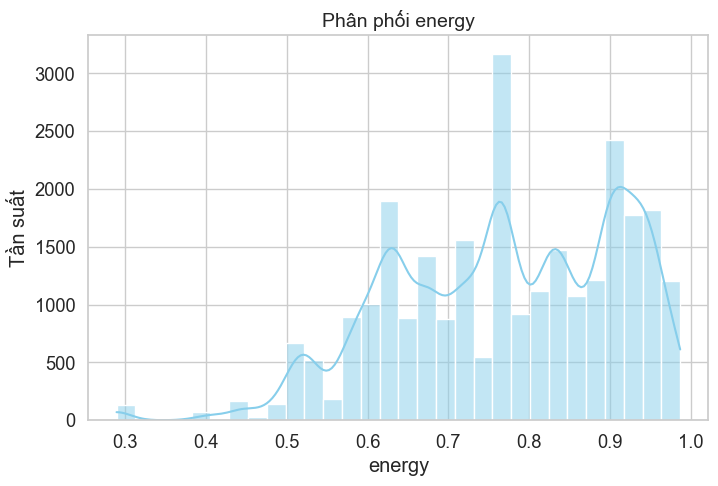
\includegraphics[width=\linewidth]{../graphics/data_top50/figure/3/EDA_japan.png}
            \\[4pt] {\small \textbf{Japan}}
        \end{minipage}
        \hfill
        \begin{minipage}{0.45\textwidth}
            \centering
            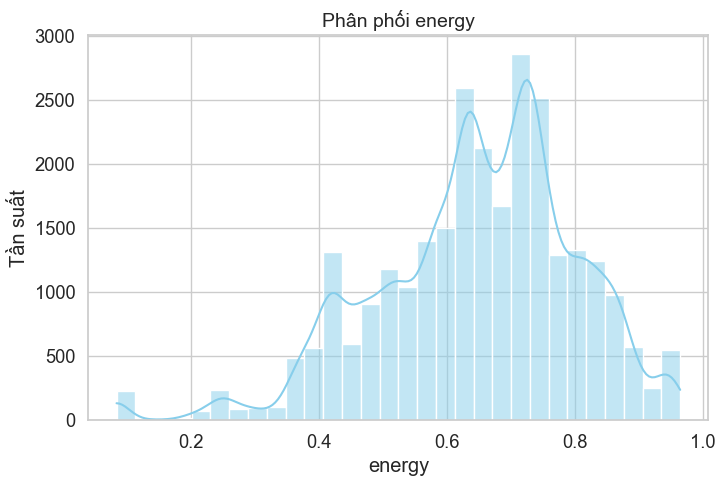
\includegraphics[width=\linewidth]{../graphics/data_top50/figure/3/EDA_world.png}
            \\[4pt] {\small \textbf{World}}
        \end{minipage}



        
        \caption{Đặc trưng energy}
        \label{fig:energy-regions}
    \end{figure}
    
        \item \textbf{Kết luận:}
        \item Tồn tại sự khác biệt rõ rệt về mức năng lượng ưa chuộng giữa các thị trường, phản ánh sự đa dạng trong văn hóa nghe nhạc và đặc tính thể loại bản địa.
        \item Phân cực rõ ràng giữa hai nhóm thị trường:
        \begin{itemize}
            \item Nhóm năng lượng cao \& đa dạng: Hầu hết các quốc gia như Argentina, France, UK, USA có phân phối energy. trải dài từ 0.2 đến 1.0 => thị hiếu âm nhạc tại đây rất đa dạng, chấp nhận cả những bài nhạc trầm lắng (energy thấp) lẫn những bài cực kỳ sôi động (energy cao).
            \item Nhóm năng lượng trung bình \& "ôn hòa": Italy và Spain có phân phối giới hạn trong khoảng 0.2 đến 0.9 => top âm nhạc tại đây có xu hướng thiếu vắng những bài hát có mức năng lượng cực cao, phù hợp với các thể loại mang tính chất nhẹ nhàng, êm dịu hơn như Pop, Ballad, hoặc Latin truyền thống.
        \end{itemize}
        \item Japan là trường hợp đặc biệt: Phân phối energy của Nhật bắt đầu từ 0.3 đến 1.0. Ngưỡng năng lượng tối thiểu cao hơn => ưa chuộng những bản nhạc có tiết tấu nhanh và sôi động ngay từ đầu, ít các bài hát có nhịp độ chậm và trầm buồn
        \item Thị trường toàn cầu (World) là sự kết hợp: Phân phối energy của World phủ rộng từ 0.2 đến 1.0, phản ánh chính xác việc nó là sự tổng hòa của tất cả các thị trường, thể hiện sự đa dạng và toàn diện nhất về mức năng lượng.
    \end{itemize}


    \item\textbf{4.2 Đặc trưng tempo}
 
           \begin{figure}[H]
        \centering
        % Dòng 1
        \begin{minipage}{0.45\textwidth}
            \centering
            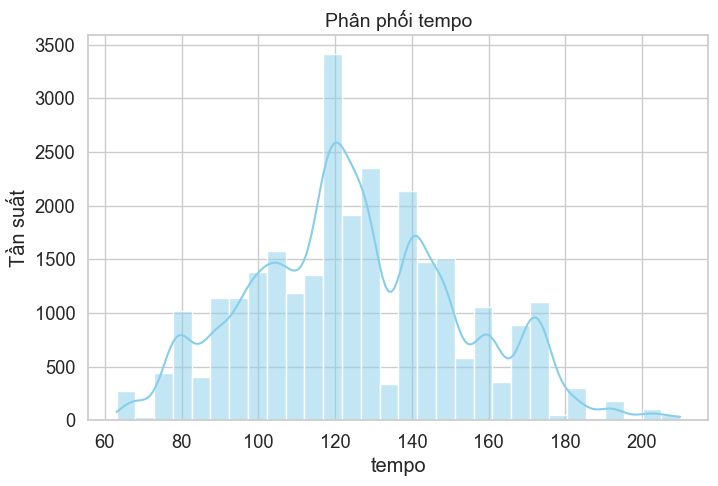
\includegraphics[width=\linewidth]{../graphics/data_top50/figure/4/EDA_uk.png}
            \\[4pt] {\small \textbf{UK}}
        \end{minipage}
        \hfill
        \begin{minipage}{0.45\textwidth}
            \centering
            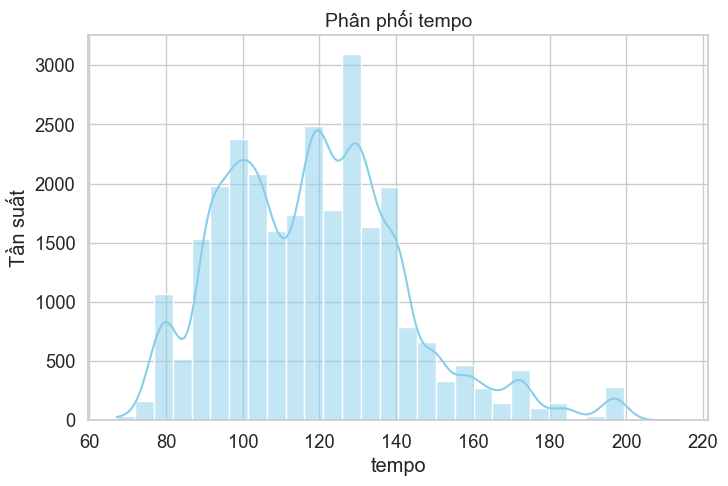
\includegraphics[width=\linewidth]{../graphics/data_top50/figure/4/EDA_italy.png}
            \\[4pt] {\small \textbf{italy}}
        \end{minipage}

        \vspace{0.4cm}

        % Dòng 2
        \begin{minipage}{0.45\textwidth}
            \centering
            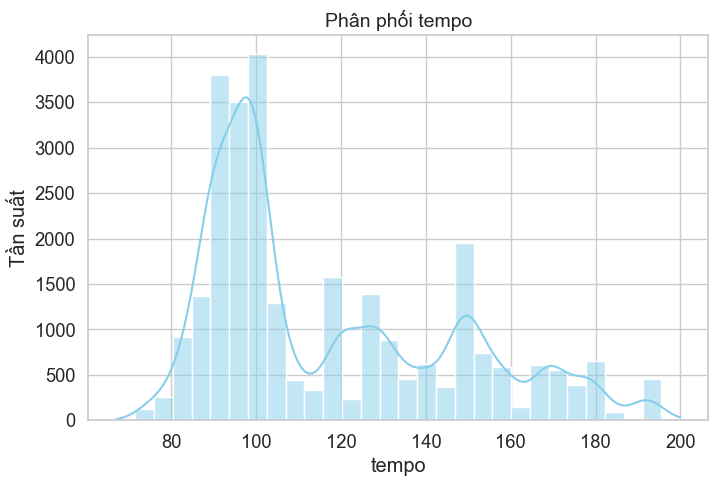
\includegraphics[width=\linewidth]{../graphics/data_top50/figure/4/EDA_argentina.png}
            \\[4pt] {\small \textbf{Argentian}}
        \end{minipage}
        \hfill
        \begin{minipage}{0.45\textwidth}
            \centering
            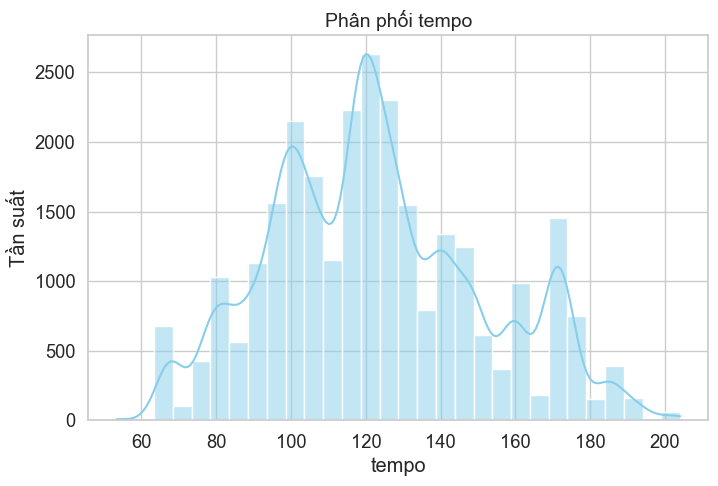
\includegraphics[width=\linewidth]{../graphics/data_top50/figure/4/EDA_world.png}
            \\[4pt] {\small \textbf{World}}
        \end{minipage}



        
        \caption{Đặc trưng tempo}
        \label{fig:energy-regions}
    \end{figure}
    

    
            \begin{itemize}
        \item \textbf{Kết luận: }

        \item Tồn tại sự tương đồng lớn về phân phối nhịp độ giữa các thị trường chủ chốt. Các nước như Argentina, Mexico, Nhật Bản (Japan) và Hàn Quốc (South Korea) có phân phối tempo gần như trùng khớp, tập trung cao ở khoảng 100-140 BPM. Điều này cho thấy một "công thức nhịp độ toàn cầu" cho các bản hit.
        \item Một số thị trường có phạm vi nhịp độ rộng hơn. Các nước như Italy, Tây Ban Nha (Spain), Pháp (France), Anh (UK), Mỹ (USA) và thị trường Thế giới (World) có phân phối trải dài từ khoảng 60 BPM đến 180-200 BPM. Sự đa dạng này phản ánh tính chất âm nhạc phong phú, bao gồm cả những bản ballad chậm rãi (tempo thấp) lẫn những bài EDM hoặc Rock sôi động (tempo cao).
        \item Nhịp độ trung bình (~80-140 BPM) là phổ biến nhất trên toàn cầu, phù hợp với các thể loại nhạc phổ biến như Pop, Rap và Dance. Phân phối của thị trường Thế giới (World) một lần nữa đóng vai trò là trung bình chuẩn mực, tổng hòa xu hướng từ tất cả các thị trường thành phần.
        
    \end{itemize}

    
 

     \item\textbf{4.3 Đặc trưng valence}
    
           \begin{figure}[H]
        \centering
        % Dòng 1
        \begin{minipage}{0.45\textwidth}
            \centering
            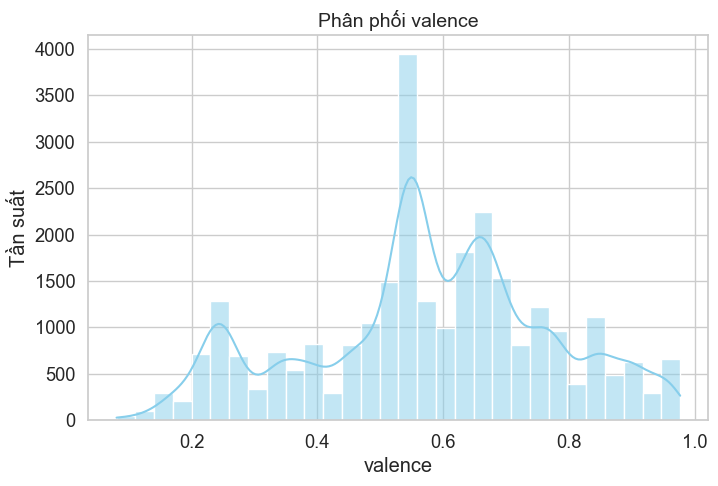
\includegraphics[width=\linewidth]{../graphics/data_top50/figure/5/EDA_spain.png}
            \\[4pt] {\small \textbf{Spain}}
        \end{minipage}
        \hfill
        \begin{minipage}{0.45\textwidth}
            \centering
            \includegraphics[width=\linewidth]{../graphics/data_top50/figure/5/EDA_japan.png}
            \\[4pt] {\small \textbf{Japan}}
        \end{minipage}

        \vspace{0.4cm}

        % Dòng 2
        \begin{minipage}{0.45\textwidth}
            \centering
            \includegraphics[width=\linewidth]{../graphics/data_top50/figure/5/EDA_usa.png}
            \\[4pt] {\small \textbf{USA}}
        \end{minipage}
        \hfill
        \begin{minipage}{0.45\textwidth}
            \centering
            \includegraphics[width=\linewidth]{../graphics/data_top50/figure/5/EDA_world.png}
            \\[4pt] {\small \textbf{World}}
        \end{minipage}



        
        \caption{Đặc trưng valence}
        \label{fig:energy-regions}
    \end{figure}
    

            
            \begin{itemize}
                \item \textbf{Kết luận: }
                \item Đa số các thị trường có phân phối valence tập trung ở mức trung bình đến cao (0.4 - 0.8). Điều này cho thấy xu hướng chung toàn cầu là ưa chuộng những bài hát mang cảm xúc tích cực, vui tươi.
        
                \item Tây Ban Nha (Spain) và Nhật Bản (Japan) là hai thị trường nổi bật với xu hướng yêu thích các bản nhạc cực kỳ tích cực. Phân phối valence của hai nước này lệch hẳn về phía giá trị cao (0.8 - 1.0), với tần suất cực lớn. Điều này đặc biệt phù hợp với các thể loại sôi động, tươi vui như Reggaeton (Tây Ban Nha) và J-pop (Nhật Bản).
        
                \item Các thị trường Âu-Mỹ (Pháp, Italy, Anh, Mỹ) có phân phối cân bằng và đa dạng hơn. Phân phối của họ trải rộng từ 0.0 đến 1.0, cho thấy sự chấp nhận đối với cả những bài hát có cảm xúc trầm lắng, u sầu (valence thấp) bên cạnh những bài hát vui vẻ. Điều này phản ánh thị hiếu âm nhạc đa chiều và có chiều sâu.
            \end{itemize}

    
    

   \item \textbf{4.4 Đặc trưng danceability}
        
           \begin{figure}[H]
        \centering
        % Dòng 1
        \begin{minipage}{0.395\textwidth}
            \centering
            \includegraphics[width=\linewidth]{../graphics/data_top50/figure/6/EDA_spain.png}
            \\[4pt] {\small \textbf{Spain}}
        \end{minipage}
        \hfill
        \begin{minipage}{0.395\textwidth}
            \centering
            \includegraphics[width=\linewidth]{../graphics/data_top50/figure/6/EDA_south_korea.png}
            \\[4pt] {\small \textbf{Korea}}
        \end{minipage}

        \vspace{0.4cm}

        % Dòng 2
        \begin{minipage}{0.395\textwidth}
            \centering
            \includegraphics[width=\linewidth]{../graphics/data_top50/figure/6/EDA_usa.png}
            \\[4pt] {\small \textbf{USA}}
        \end{minipage}
        \hfill
        \begin{minipage}{0.395\textwidth}
            \centering
            \includegraphics[width=\linewidth]{../graphics/data_top50/figure/6/EDA_world.png}
            \\[4pt] {\small \textbf{World}}
        \end{minipage}



        
        \caption{Đặc trưng danceability}
        \label{fig:energy-regions}
    \end{figure}
    

            
            \begin{itemize}
                \item \textbf{Kết luận: }
                
                \item Nhóm ưa chuộng tính nhảy múa rất cao: Các quốc gia như Argentina, Italy, Japan, Mexico và Tây Ban Nha (Spain) có phân phối danceability rất hẹp, tập trung ở khoảng 0.6 - 0.9. Điều này cho thấy các bài hát ở đây gần như bắt buộc phải có nhịp điệu dễ nhảy theo, phù hợp với các thể loại như Reggaeton, Latin Pop hay EDM.
        
                \item Nhóm linh hoạt hơn: Các thị trường Pháp (France), Hàn Quốc (South Korea), Anh (UK), Mỹ (USA) và Thế giới (World) có phân phối rộng hơn, từ 0.2 đến 1.0. Mặc dù vẫn nghiêng về các bài hát dễ nhảy, họ vẫn chấp nhận những bài hát ít tính nhảy múa hơn (ví dụ: ballad, nhạc acoustic), cho thấy thị hiếu đa dạng.
        
                \item Phân phối của thị trường Thế giới (World)  cho thấy sự cân bằng, nhưng vẫn nghiêng nhiều về nhóm các bài hát có danceability cao, chứng tỏ đây là một xu hướng chủ đạo.
            \end{itemize}

    
    
\end{itemize}


\textbf{5. So sánh nhóm }
\begin{itemize}
    \item \textbf{5.1 Tỷ lệ Explicit}
       
    % \begin{figure}[H]
    %     \centering
    %     % Dòng 1
    %     \begin{minipage}{0.3\textwidth}
    %         \centering
    %         \includegraphics[width=\linewidth]{../graphics/data_top50/34/EDA_japan.png}
    %         \\[4pt] {\small \textbf{Japan}}
    %     \end{minipage}
    %     % \hfill
    %     % \begin{minipage}{0.3\textwidth}
    %     %     \centering
    %     %     \includegraphics[width=\linewidth]{../graphics/data_top50/34/EDA_argentina.png}
    %     %     \\[4pt] {\small \textbf{Argentina}}
    %     % \end{minipage}

    %     % \vspace{0.2cm}

    %     % Dòng 2
    %     % \begin{minipage}{0.3\textwidth}
    %     %     \centering
    %     %     \includegraphics[width=\linewidth]{../graphics/data_top50/34/EDA_usa.png}
    %     %     \\[4pt] {\small \textbf{USA}}
    %     % \end{minipage}
    %     % % \hfill
    %     % \begin{minipage}{0.3\textwidth}
    %     %     \centering
    %     %     \includegraphics[width=\linewidth]{../graphics/data_top50/34/EDA_world.png}
    %     %     \\[4pt] {\small \textbf{World}}
    %     % \end{minipage}



        
    %     \caption{Tỷ lệ Explicit}
    %     \label{fig:energy-regions}
    % \end{figure}


\begin{figure}[H]
    \centering
    % === Cột bên trái ===
    \begin{minipage}{0.38\textwidth}
        \centering
        \includegraphics[width=\linewidth]{../graphics/data_top50/34/EDA_japan.png}
        \\[4pt] {\small \textbf{Japan}}
    \end{minipage}
    \hfill
    % === Cột bên phải ===
    \begin{minipage}{0.38\textwidth}
        \centering
        \includegraphics[width=\linewidth]{../graphics/data_top50/34/EDA_world.png}
        \\[4pt] {\small \textbf{World}}
    \end{minipage}

    \caption{So sánh tỷ lệ Explicit }
    \label{fig:explicit-japan-world}
\end{figure}

    
           \begin{itemize}
        \item \textbf{Kết luận:}
        \item Tồn tại sự khác biệt văn hóa cực kỳ lớn giữa các thị trường trong việc chấp nhận nội dung explicit.
        \item Nhật Bản và Hàn Quốc với tỷ lệ bài hát clean áp đảo tuyệt đối (> 90 \%). Điều này cho thấy một tiêu chuẩn văn hóa và giải trí rất khắt khe, phù hợp với các thể loại nhạc đại chúng như J-pop và Anime.

       \item Các thị trường châu Á và châu Âu thể hiện sự phân cực rõ rệt:

      \item Argentina là thị trường có tỷ lệ bài hát explicit cao nhất (68.3 \% ), cho thấy sự thống trị của các thể loại như Argentine Trap và Reggaeton, nơi nội dung explicit là một phần của văn hóa âm nhạc.

      \item Các thị trường lớn còn lại (Italy, Mexico, Spain, UK, USA, World) có tỷ lệ gần như cân bằng (~50/50). Điều này cho thấy sự chấp nhận và cạnh tranh song hành giữa hai dòng nhạc, phản ánh sự đa dạng và phân hóa trong thị hiếu của người nghe.
    \end{itemize}

    \item \textbf{5.2 Solo vs Colab}
        
    \begin{figure}[H]
        \centering
        % === Cột bên trái ===
        \begin{minipage}{0.38\textwidth}
            \centering
            \includegraphics[width=\linewidth]{../graphics/data_top50/figure/21/EDA_usa.png}
            \\[4pt] {\small \textbf{USA}}
        \end{minipage}
        \hfill
        % === Cột bên phải ===
        \begin{minipage}{0.38\textwidth}
            \centering
            \includegraphics[width=\linewidth]{../graphics/data_top50/figure/21/EDA_spain.png}
            \\[4pt] {\small \textbf{Spain}}
        \end{minipage}

        % \caption{So sánh tỷ lệ Explicit }
        % \label{fig:explicit-japan-world}
    \end{figure}


    \begin{figure}[H]
        \centering
        % === Cột bên trái ===
        \begin{minipage}{0.38\textwidth}
            \centering
            \includegraphics[width=\linewidth]{../graphics/data_top50/figure/21/EDA_japan.png}
            \\[4pt] {\small \textbf{Japan}}
        \end{minipage}
        \hfill
        % === Cột bên phải ===
        \begin{minipage}{0.38\textwidth}
            \centering
            \includegraphics[width=\linewidth]{../graphics/data_top50/figure/21/EDA_world.png}
            \\[4pt] {\small \textbf{World}}
        \end{minipage}

        \caption{So sánh tỷ lệ Explicit }
        \label{fig:explicit-japan-world}
    \end{figure}
    

    % \begin{figure}[H]
    %     \centering
    %     % Dòng 1
    %     \begin{minipage}{0.45\textwidth}
    %         \centering
    %         \includegraphics[width=\linewidth]{}
    %         \\[4pt] {\small \textbf{USA}}
    %     \end{minipage}
    %     \hfill
    %     \begin{minipage}{0.45\textwidth}
    %         \centering
    %         \includegraphics[width=\linewidth]{}
    %         \\[4pt] {\small \textbf{Spain}}
    %     \end{minipage}

    %     \vspace{0.4cm}

    %     % Dòng 2
    %     \begin{minipage}{0.45\textwidth}
    %         \centering
    %         \includegraphics[width=\linewidth]{}
    %         \\[4pt] {\small \textbf{Japan}}
    %     \end{minipage}
    %     \hfill
    %     \begin{minipage}{0.45\textwidth}
    %         \centering
    %         \includegraphics[width=\linewidth]{g}
    %         \\[4pt] {\small \textbf{World}}
    %     \end{minipage}



        
    %     \caption{Tỷ lệ Solo vs Colab}
    %     \label{fig:energy-regions}
    % \end{figure}
    
            \begin{itemize}
                 \item \textbf{Kết luận:}
                \item Tỷ lệ bài hát Solo chiếm ưu thế tuyệt đối trên toàn cầu => nghệ sĩ cá nhân vẫn có sức hút và khả năng thống trị các bảng xếp hạng lớn.
                \item Tồn tại sự khác biệt lớn về văn hóa âm nhạc giữa các thị trường:
                      \begin{itemize}
                          \item Nhật Bản và Hàn Quốc là thị trường đề cao tính cá nhân rõ rệt nhất, với tỷ lệ bài hát Solo chiếm tới 95.5 \%. Điều này phù hợp với đặc trưng của J-pop, K-pop, nơi các nghệ sĩ solo thường được xây dựng hình tượng mạnh mẽ.
                          \item Các thị trường Mỹ Latin (Argentina, Mexico, Tây Ban Nha) có tỷ lệ Collab (hợp tác) cao nhất, dao động từ ~37 \% đến 46\%. Điều này phản ánh đặc tính cộng đồng và xu hướng kết hợp trong các thể loại âm nhạc phổ biến tại đây như Reggaeton, Latin Trap.
                          \item Các thị trường Âu-Mỹ (Mỹ, Anh, Pháp, Italy) có tỷ lệ Solo rất cao (từ 69.7\% đến 87.3\%), cho thấy sự thống trị của các ngôi sao solo trong làng nhạc đại chúng.
                          
                          
                      \end{itemize}
                \item Ở Thế giới, Bài hát Solo chiếm ưu thế rõ rệt (82.0\%), cho thấy sức hút và khả năng thống trị bảng xếp hạng toàn cầu của các nghệ sĩ cá nhân.
             \end{itemize}
\end{itemize}



























